
% CHAPTER 4

\chapter{SIMULATION ENVIRONMENT $\&$ RESULTS}
\label{chp:simulation}


\externaldocument{chapter1}
\externaldocument{chapter2}
\externaldocument{chapter3}






	In this section the simulation environment is illustrated and the results are analyzed and discussed in detail for the local positioning system design and formation control system design. Three different methods of formation control system which are presented in Section \ref{chp:Methodology} are evaluated and compared with each other. Simulations are handled in the environment of Gazebo simulator with a swarm of 50 agents which includes three different types of robots. The main system frequncy in which each agent propogate their state vectors, calculate artificial forces and make goal state assignments is determined as 2Hz due to the bandwith of the inner loop controllers which is discussed in Section \ref{lqr_design}. 
	\subsection{Simulation Environment}
    Block diagram of the simulation environment is illustrated in Figure \ref{simulation_env_ref}.
    
    
    	\begin{figure}[H]
    		\caption{Simulation Environment} \label{simulation_env_ref}
    		\centering
    		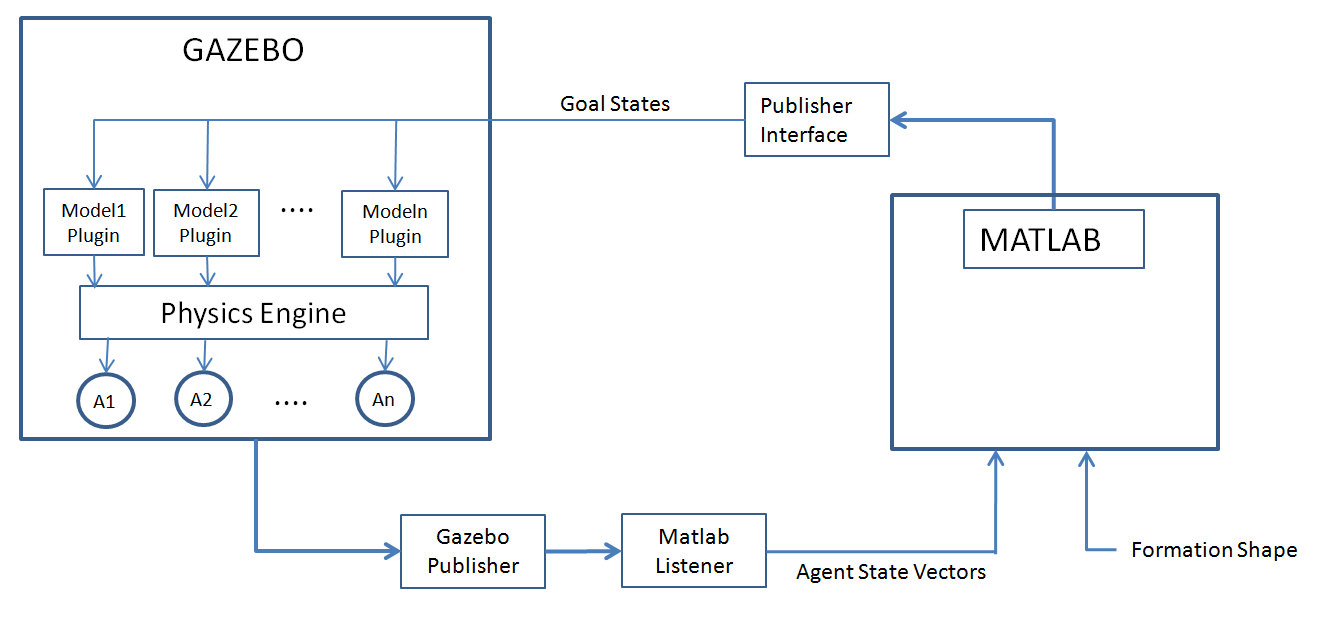
\includegraphics[scale = 0.50]{environment}
    	\end{figure}
    

    
	Gazebo is an open source multi robot simulator developed by OSRF(Open Source Robotics Foundation). It has multiple physics engine ODE (Open Dynamics Engine), Bullet, DART(Dynamic Animation and Robotics Toolkit) and Simbody. It can execute simulations with multiple agents in an environment that is fully determined by the user. The dynamics and the physical properties of the robots are determined by the user. It can be integrated with Robot Operating System(ROS)
    Shape partitioning algorithms are executed in Matlab environment and  potential goal states are published over a network socket. A plugin working in Gazebo environment listens the packets sent by Matlab and parse the data for each agent. Agents have their own plugins that listens goal states and execute their decision process algorithms. These plugins also have controller algorithms to make the agents reached to the goal states they have assigned. Dynamics of the agents are handled in the physics engines of the Gazebo simulator. The state vectors of the agents are published with a plugin from the Gazebo simulator and these state datas are used in the shape partitioning algorithms together with the formation shapes demanded by the user.   The environment is chosen as a rough 3D territory and each agent have different interactions with the environment with different mass and friction characteristics.
    


	
	\subsection{LPS  Design}
In the LPS design, the main aim is to design an architecture in which every agent can localize itself with the help of the position agents which have positioning sensors on their boards. With the help of DSDV algorithms, each individual agent assign itself to the cluster of position agent with minimum number of hops in the network which is discussed in Section-xx. A sample output of this algorithm at an instant time during simulations is illustrated in Figure-xx. 
	
		\begin{figure}[H]
			\caption{Cluster Assignments of the Agents}
		\centerline{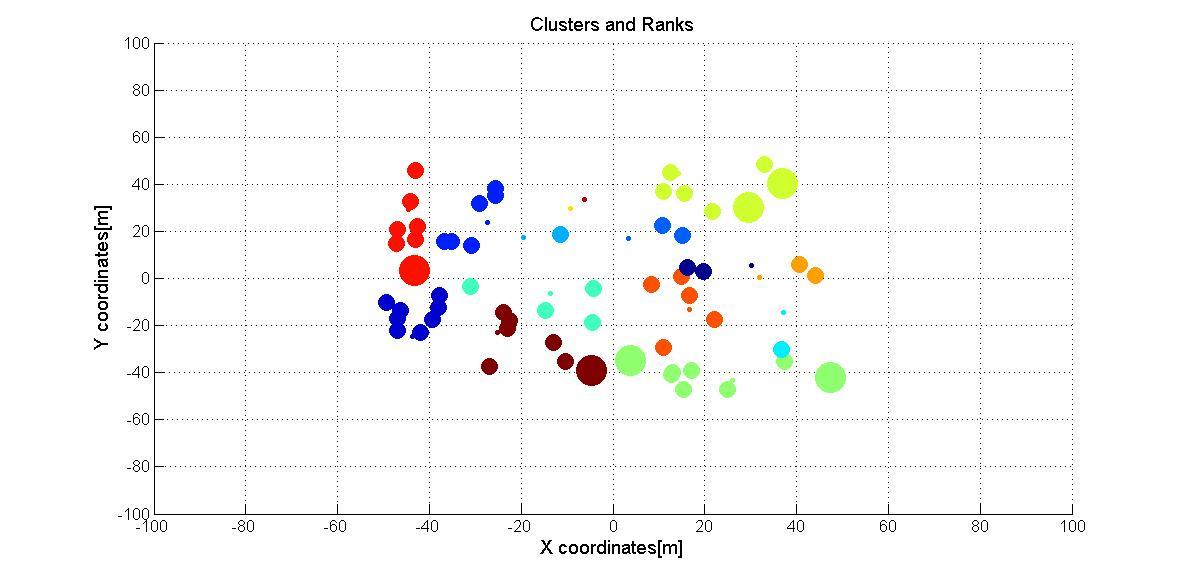
\includegraphics[scale = 0.4]{Clusters_Ranks_1}}
			\end{figure} 
	Agents with the same colors are assigned to same clusters at this instant time and their size represents the rank number of each agent at that cluster which is determined with the number of hops. It is important to notice that agents are assigned to the clusters of the position agents with minimum number of hops rather than the minimum distance since it is expected to have greater errors on position data with the increasing number of ranks because of the cumulative error effect. This assumption is supported with the simulation experiments and results are presented in Figure-xx. 
The agents which are not directly get into trilateration process with the position agents (i.e. agents with rank greater than 2) have to localize themselves with the help of their neighbor with lower ranks,thus their position data will include the errors of the localization process of their neighbors. This situation is illustrated in Figure-x, total error is increasing cumulatively with the number of rank. 
	

			\begin{figure}[H]
				\caption{Total Error on Position Data with Respect to Ranks}
				\centerline{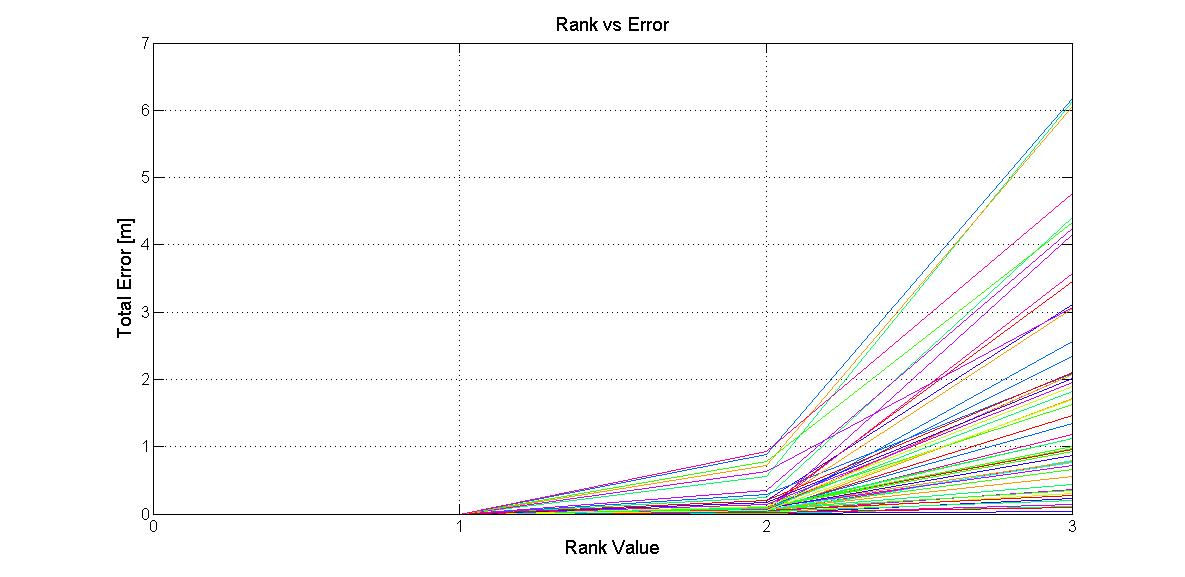
\includegraphics[scale = 0.4]{Rank_vs_Error}}
		\end{figure} 
	
The state propogation period which is discussed in Section-xx is determined as 2Hz as equal to the main system frequency since the new position datas for the formation control system are required to be determined with this rate. 	As discussed in Section-xx, a localization timer is proposed to handle the DSDV algorithm and trilateration process which will provide a greater execution period than the propogation process of the states with the help of inertial measurements. It is obvious that the state variables will be drifting with the increasing time because of the measurement and process noise in propogation process unless they are not corrected with the external measurements, so it is possible to determine a minimum execution period of this trilateration process to satisfy an error band in the state variables. 
		
		
		\begin{figure}[H]
			\caption{Total Error with Localization Timer Period of 3 Seconds}
			\centerline{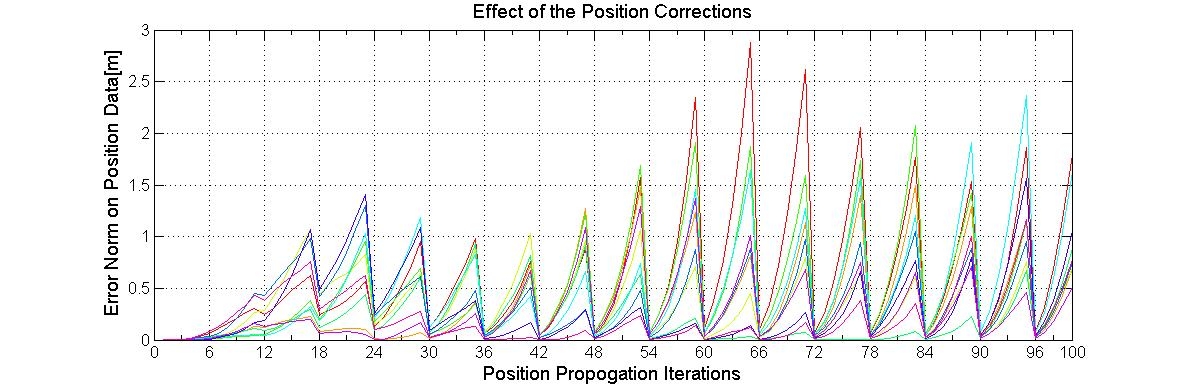
\includegraphics[scale = 0.4]{Error-0,5Prop-3Update}}
		\end{figure} 
		
				\begin{figure}[H]
					\caption{Total Error with Localization Timer Period of 5 Seconds}
					\centerline{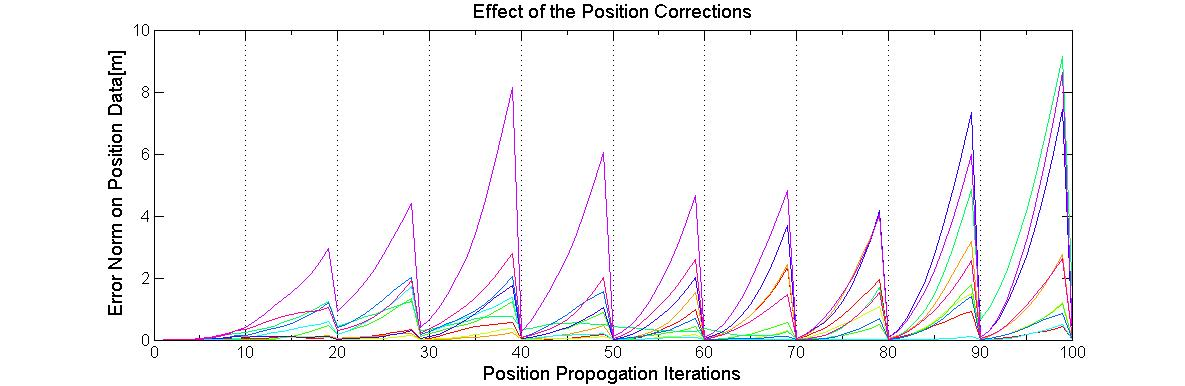
\includegraphics[scale = 0.4]{Error-0,5Prop-5Update}}
				\end{figure} 

				\begin{figure}[H]
					\caption{Total Error with Localization Timer Period of 8 Seconds}
					\centerline{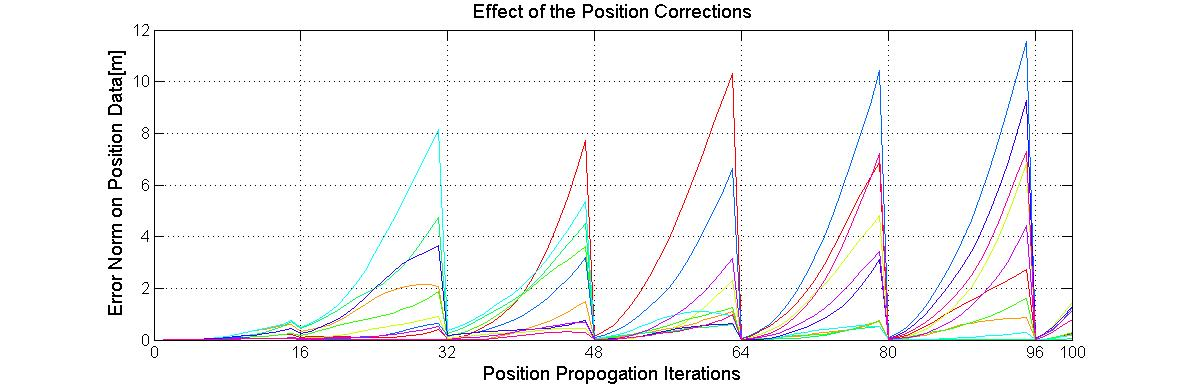
\includegraphics[scale = 0.4]{Error-0,5Prop-8Update}}
				\end{figure} 		
		
		
It is clear that the total error norm on position datas are decreased dramatically with the localization period which equals to 6 iterations for 3 seconds period, 10 iterations for 5 seconds and 16 iterations for 8 seconds period. The peak values on the error norms are always observed at the iterations just before the localization process. It can be concluded that the peak values on the error norms are greatly related with the localization period and they have greater values with the increasing number of this period. The maximum error norm is below 3 meters with localization period of 3 seconds, below 10 meters with localization period of 5 seconds and below 12 meters with localization period of 8 seconds. It is decided  that the error norm of 3 meters is the maximum tolerable value for the formation control system and the localization period is determined as 3 seconds. 

The performance of the LPS design is tested in simulations with different conditions in which swarm is propogating to a desired formation shape or agents are keeping their positions in a given formation shapes.  In both cases, it is observed that the position datas of the agents are drifted with an increasing error between two  sequential localization process. A sample case for this situation is illustrated in Figure -xx


		
		\begin{figure}[H]
\caption{Local Positioning System}
\centering
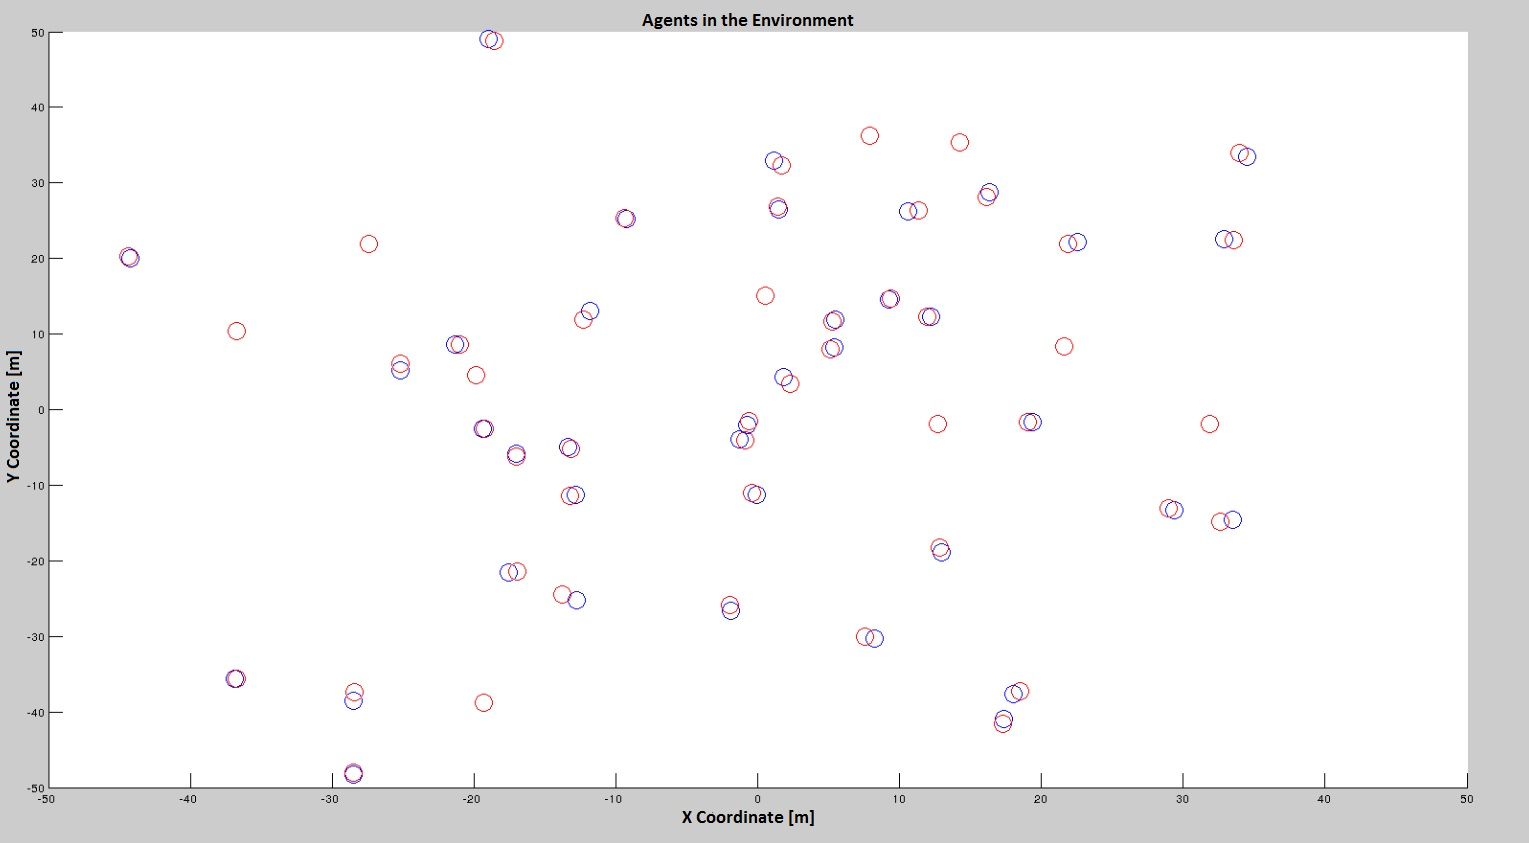
\includegraphics[scale = 0.65]{Pozisyon_1_Hatali}
\label{fig:lps}
\end{figure}

			\begin{figure}[H]
				\caption{Positions of the Agents After Localization Process \\
					(Red Circles: Estimated Positions ; Blue Circles: Real Positions)}
				\centerline{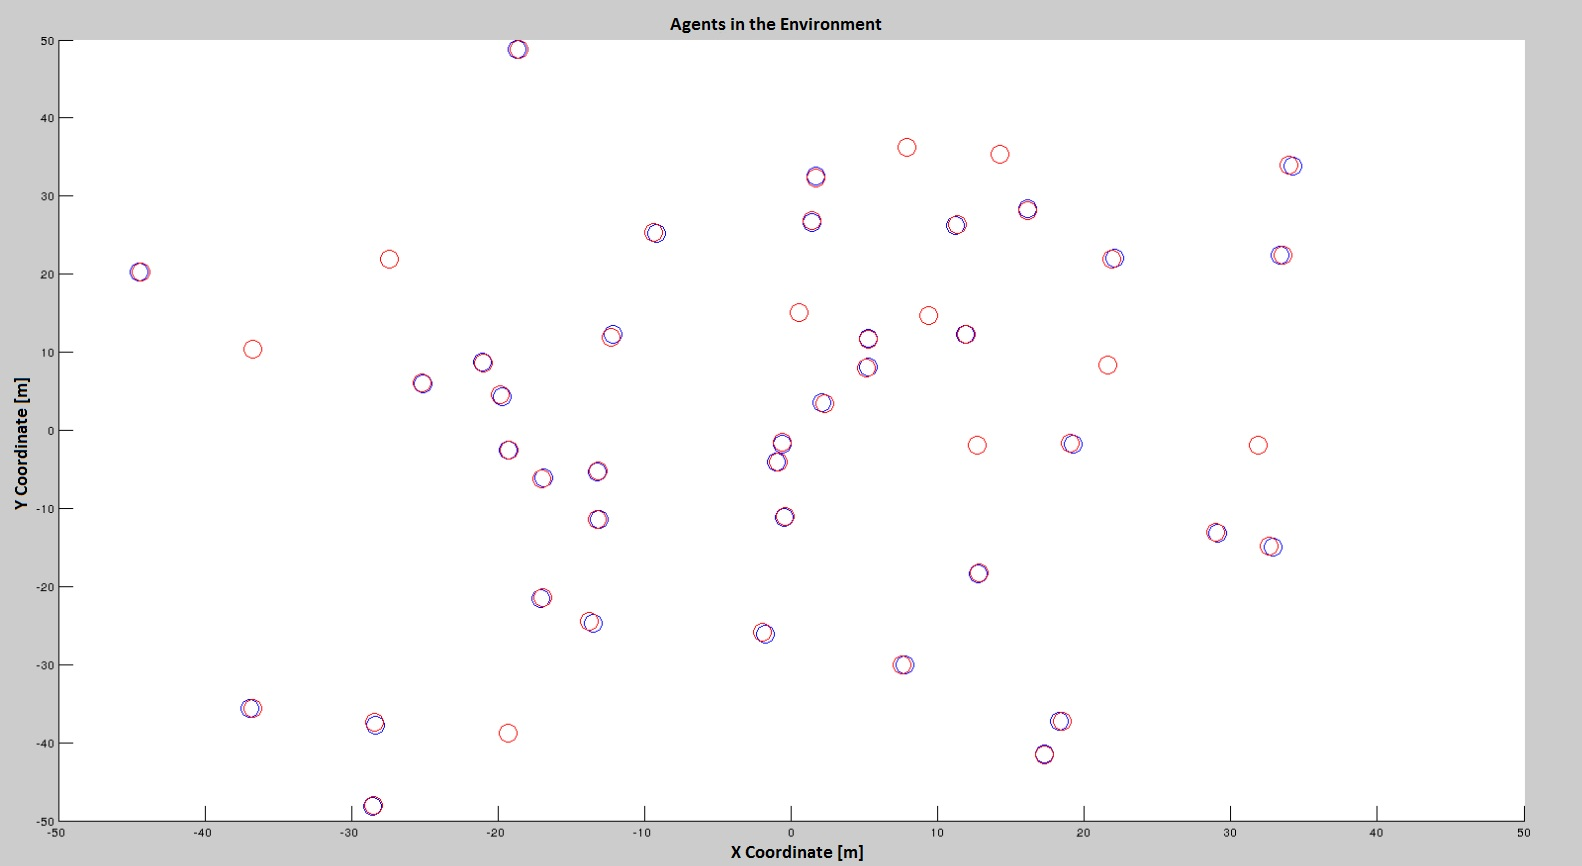
\includegraphics[scale = 0.30]{Pozisyon-1-Duzeltilmis}}
			\end{figure} 
		
		Handling procedures of the lost agents are presented in Section-xx. Agents which do not have three neighbors around itselves will get into the 'Lost' mode, and if  they miss three localization process they will get into 'Come Home' mode. When an agent have 'Come Home' mode, it will try to reach the center of formation to increase the possibility to meet some neighbors to localize itself as discussed in Section-xx. A simulation result in which two agents cannot have three neighbors around themselves and get into 'Lost' mode and 'Come Home' modes  is presented in Figure -xx and Figure-xx respectively.
		
			\begin{figure}[H]
				\caption{Agents will be in 'Lost' Mode When They Do Not Have 3 Neighbors}
				\centerline{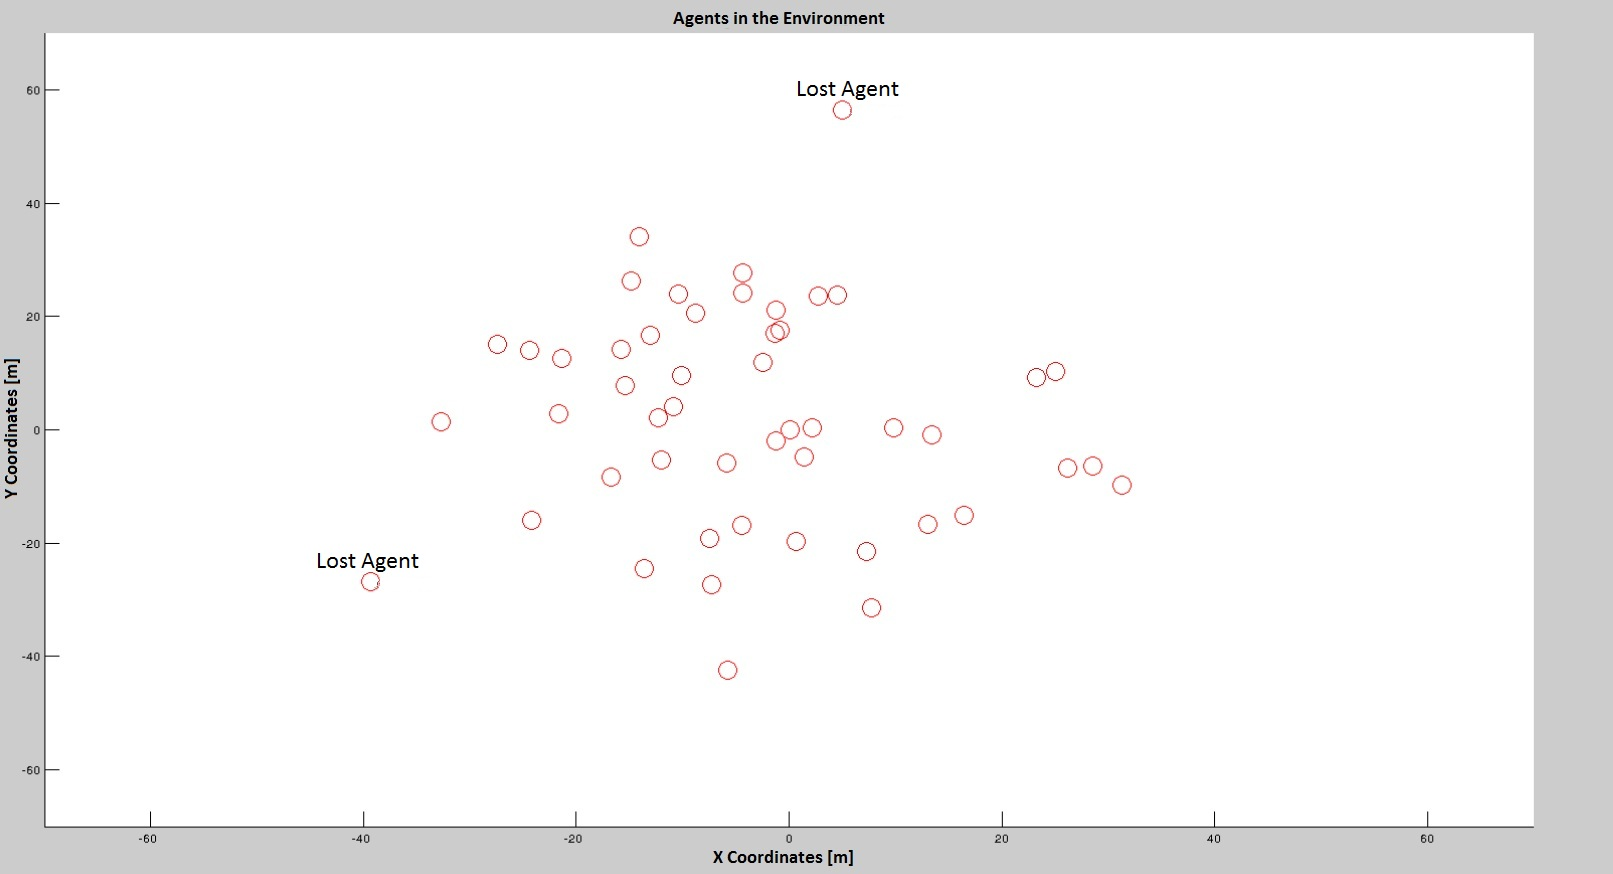
\includegraphics[scale = 0.30]{Lost-2-2}}
			\end{figure} 

			\begin{figure}[H]
				\caption{Agents will be in 'Come Home' Mode When They Miss Localization Process for 3 Times}
				\centerline{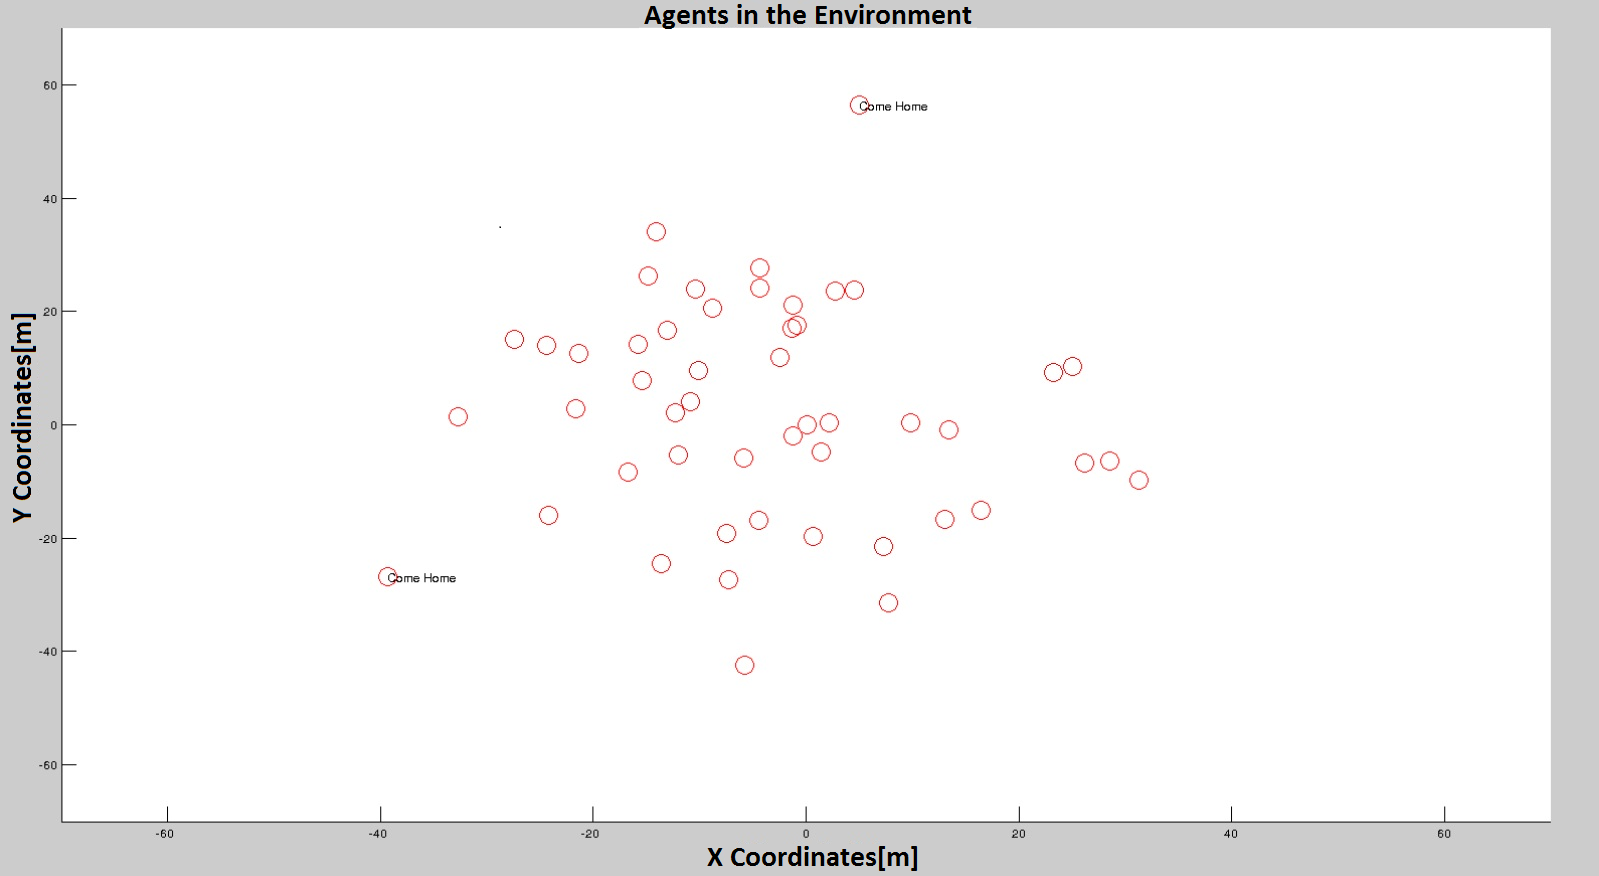
\includegraphics[scale = 0.30]{Lost-2-3}}
			\end{figure} 		
		
		
		
		\subsection{FORMATION CONTROL SYSTEM}
  Three dıfferent approaches of which the details are presented is Section-xx are evaluated according to their settling times, mesh qualities and energy consumptions. 
  \subsubsection{Mesh Qualities} 
  Mesh qualities is a measure of how the agents homogenously distributed while covering the desired formation shape. Basically, two different types of quality measurents defined in Section-xx are used to evaluate the performance of the formation control methods, topological mesh irregularity $\epsilon_t$ and geometrical mesh irregularity $\epsilon_g$ . Monte Carlo simulations with 1000 iterations are handled for the same formations shapes with different initial conditions of the agents in the environment. Sample outputs for three different types of formation control algorithms are illustrated in the following Figures
  
		
		
		\begin{figure}[H]
			\caption{Formation Shape 1 with Artificial Forces Methods:$\epsilon_t = 2.1$ and $\epsilon_g = 0.32$}
			\centerline{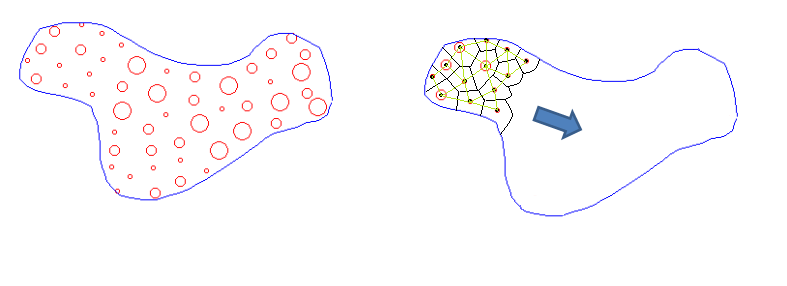
\includegraphics[scale = 0.70]{Artificial_Forces_Mesh_1}}
		\end{figure} 		
				\begin{figure}[H]
					\caption{Formation Shape 2 with Artificial Forces Methods:$\epsilon_t = 2.6$ and $\epsilon_g = 0.4$}
					\centerline{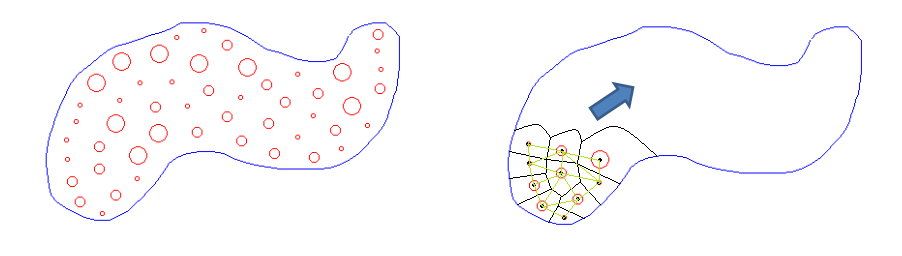
\includegraphics[scale = 0.65]{Artificial_Forces_Mesh_2}}
				\end{figure} 		
		
				\begin{figure}[H]
					\caption{Formation Shape 1 with Bubble Packing Method:$\epsilon_t = 2.1$ and $\epsilon_g = 0.24$}
					\centerline{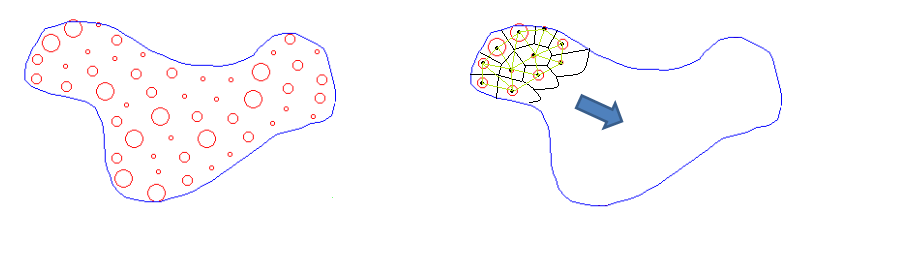
\includegraphics[scale = 0.70]{Bubble_Packing_Mesh_1}}
				\end{figure} 	
						\begin{figure}[H]
							\caption{Formation Shape 2 with Bubble Packing Method:$\epsilon_t = 2.3$ and $\epsilon_g = 0.28$}
							\centerline{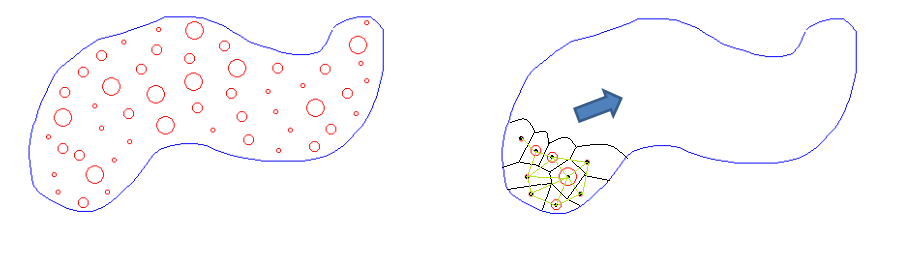
\includegraphics[scale = 0.65]{Bubble_Packing_Mesh_2}}
						\end{figure} 			
						\begin{figure}[H]
							\caption{Formation Shape 1 with Randomized Fractals Method:$\epsilon_t = 2.7$ and $\epsilon_g = 0.65$}
							\centerline{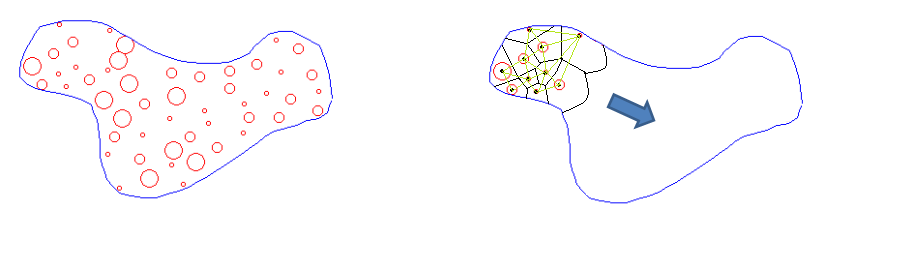
\includegraphics[scale = 0.70]{Randomized_Fractals_Mesh_1}}
						\end{figure} 	
						\begin{figure}[H]
							\caption{Formation Shape 2 with Randomized Fractals Method:$\epsilon_t = 3.1$ and $\epsilon_g = 0.62$}
							\centerline{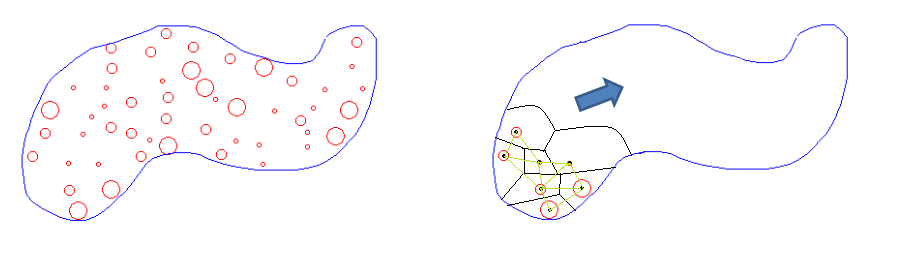
\includegraphics[scale = 0.65]{Randomized_Fractals_Mesh_2}}
						\end{figure} 	
		It is obvious that Randomized Fractals method have the worst mesh performance due the its randomized assignment of goal states into the formation shape. Bubble Packing and Artificial Forces methods give similar results since they have an analogy in their approaches of implementing inter member/bubble forces which makes the agents distributed in the formation shape more homogenously. Artificial force method applies this intermember forces directly to the agents in real time while Bubble Packing method use this kind of force on artificial bubbles to partition the shape into goal states. Monte Carlo simulations with 1000 iterations for both formation shapes are handled and the results are illustrated in Figure -x1 -x2 . Randomized Fractals method have greater mean values for both topological and geometrical mesh irregularities as expected.  Bubble Packing and Artificial Forces methods have similar performances on Mesh quality.
		
		
		
								\begin{figure}[H]
									\caption{Formation Shape 1 Topological Mesh Irregularities:}
									\centerline{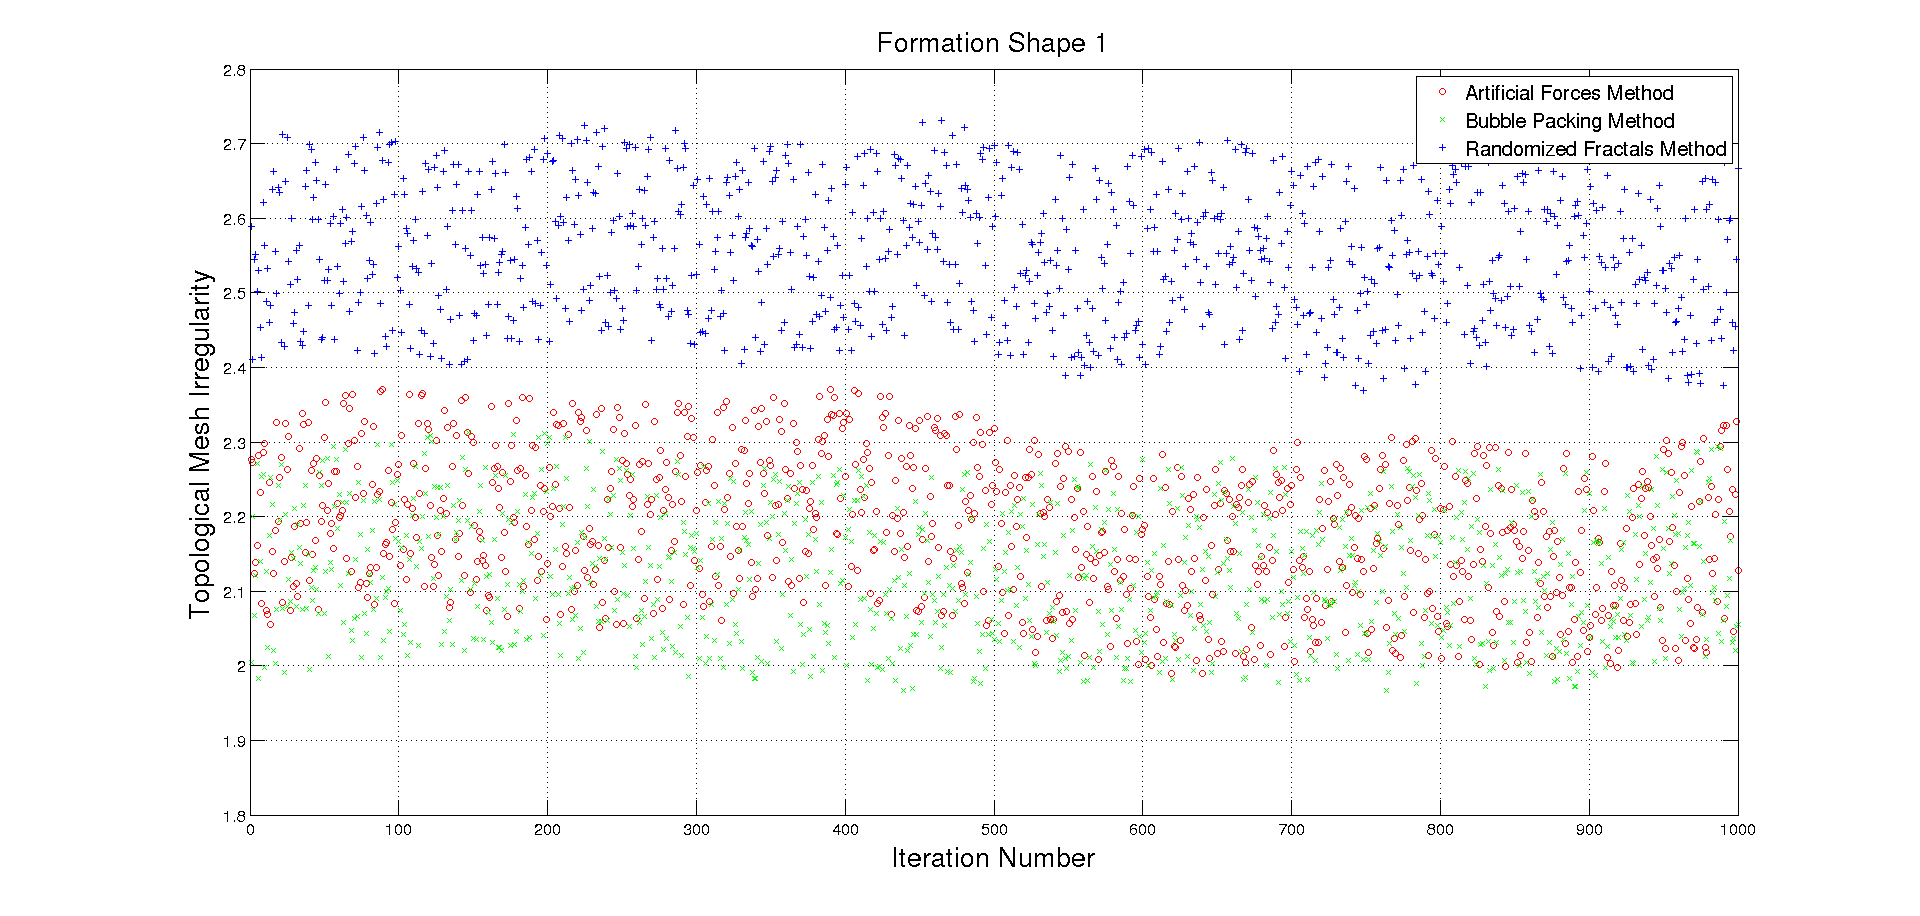
\includegraphics[scale = 0.45]{Topological_Irr_1}}
								\end{figure} 	
		
				\begin{figure}[H]
					\caption{Formation Shape 1 Geometrical Mesh Irregularities:}
					\centerline{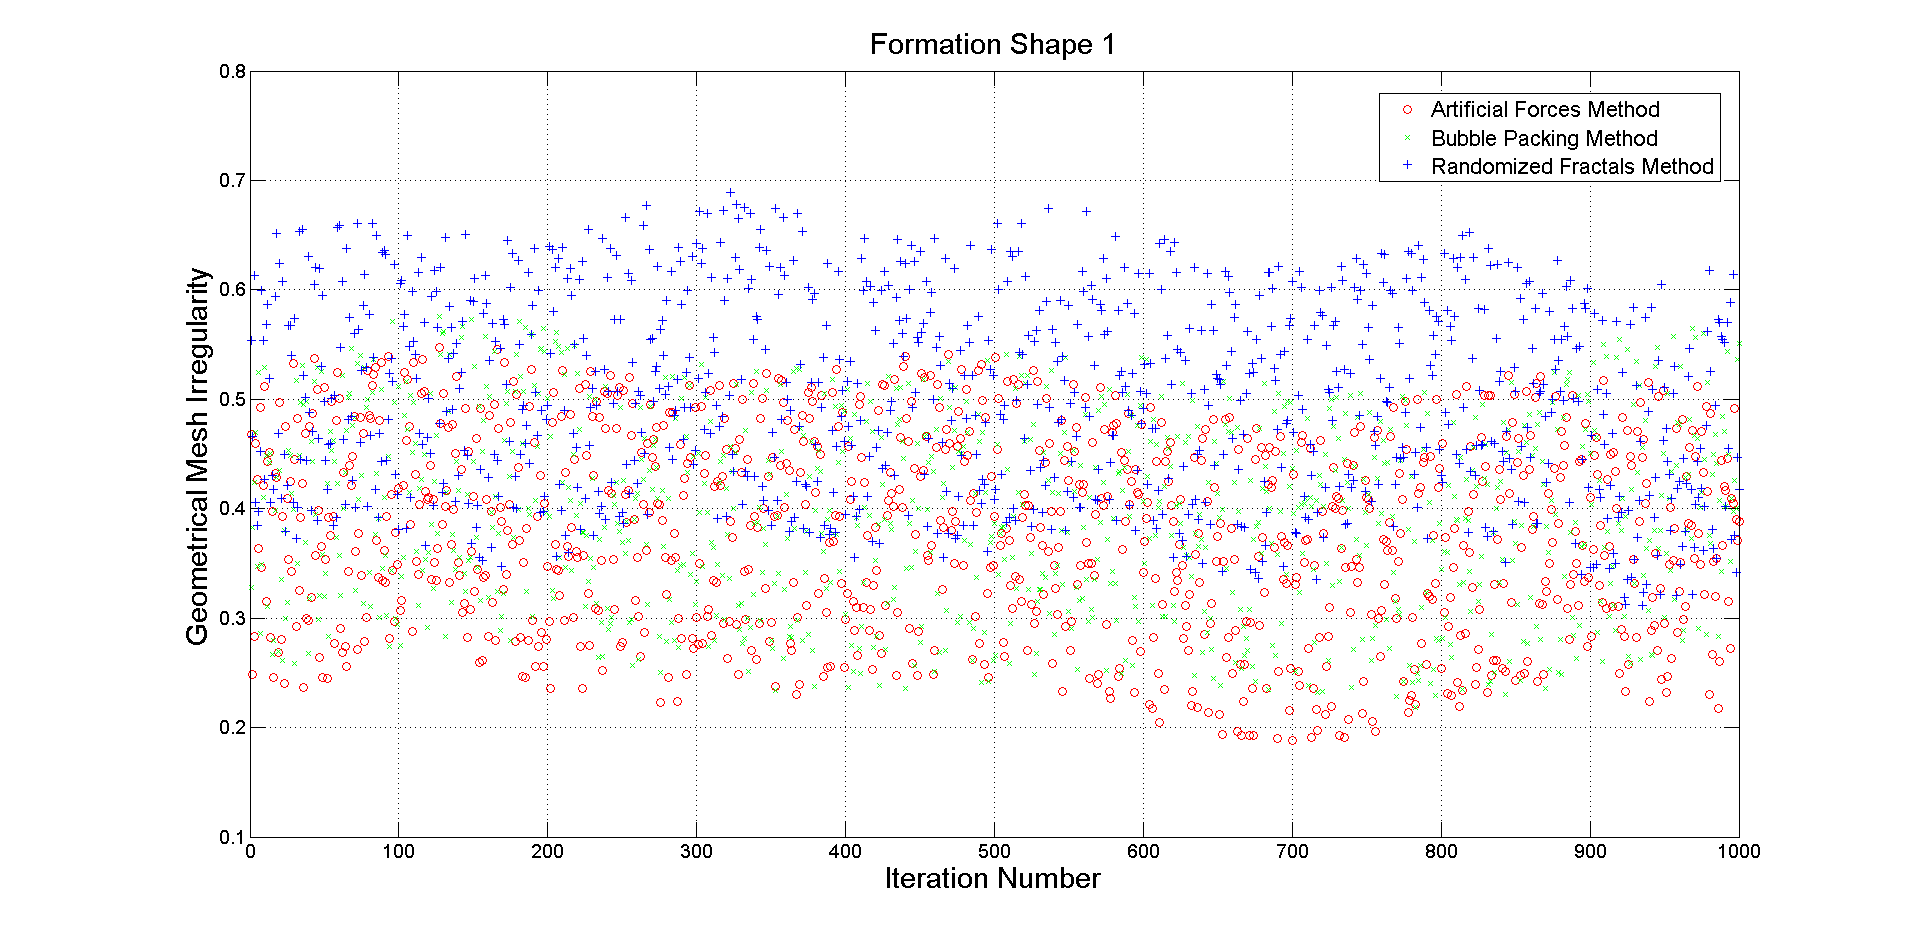
\includegraphics[scale = 0.45]{Geometrical_Irr_1}}
				\end{figure} 	

				\begin{figure}[H]
					\caption{Formation Shape 2 Topological Mesh Irregularities:}
					\centerline{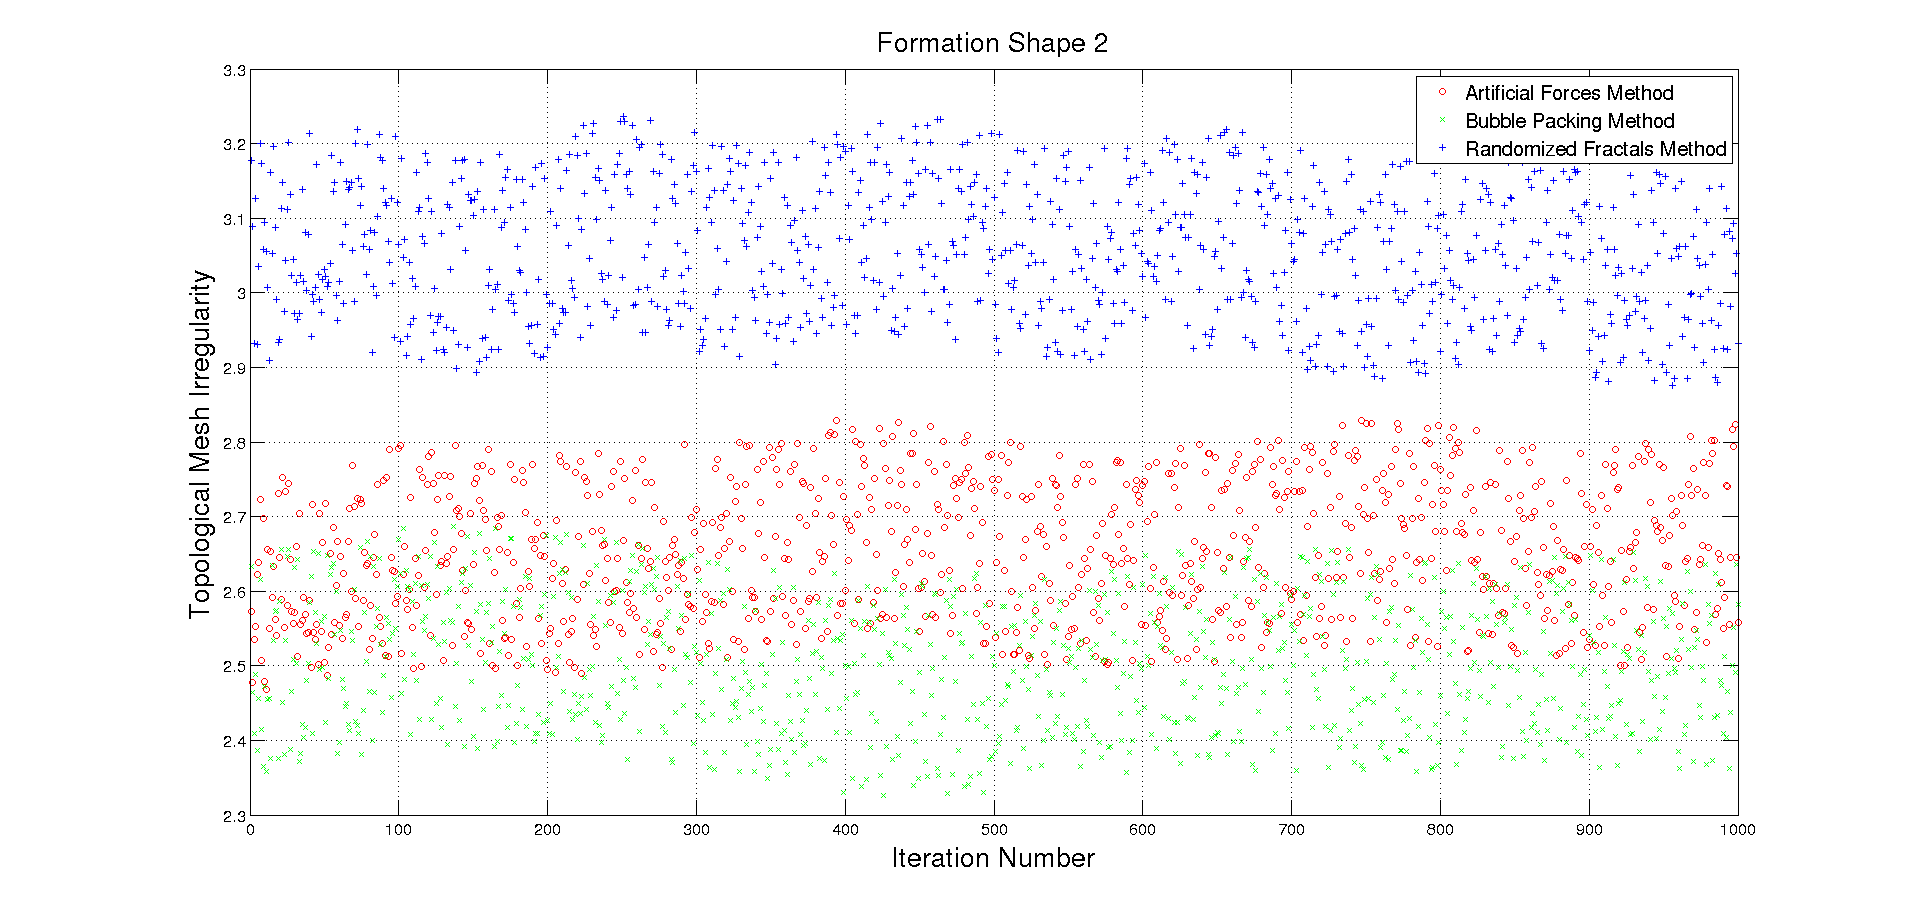
\includegraphics[scale = 0.45]{Topological_Irr_2}}
				\end{figure} 	
				
								\begin{figure}[H]
									\caption{Formation Shape 2 Geometrical Mesh Irregularities:}
									\centerline{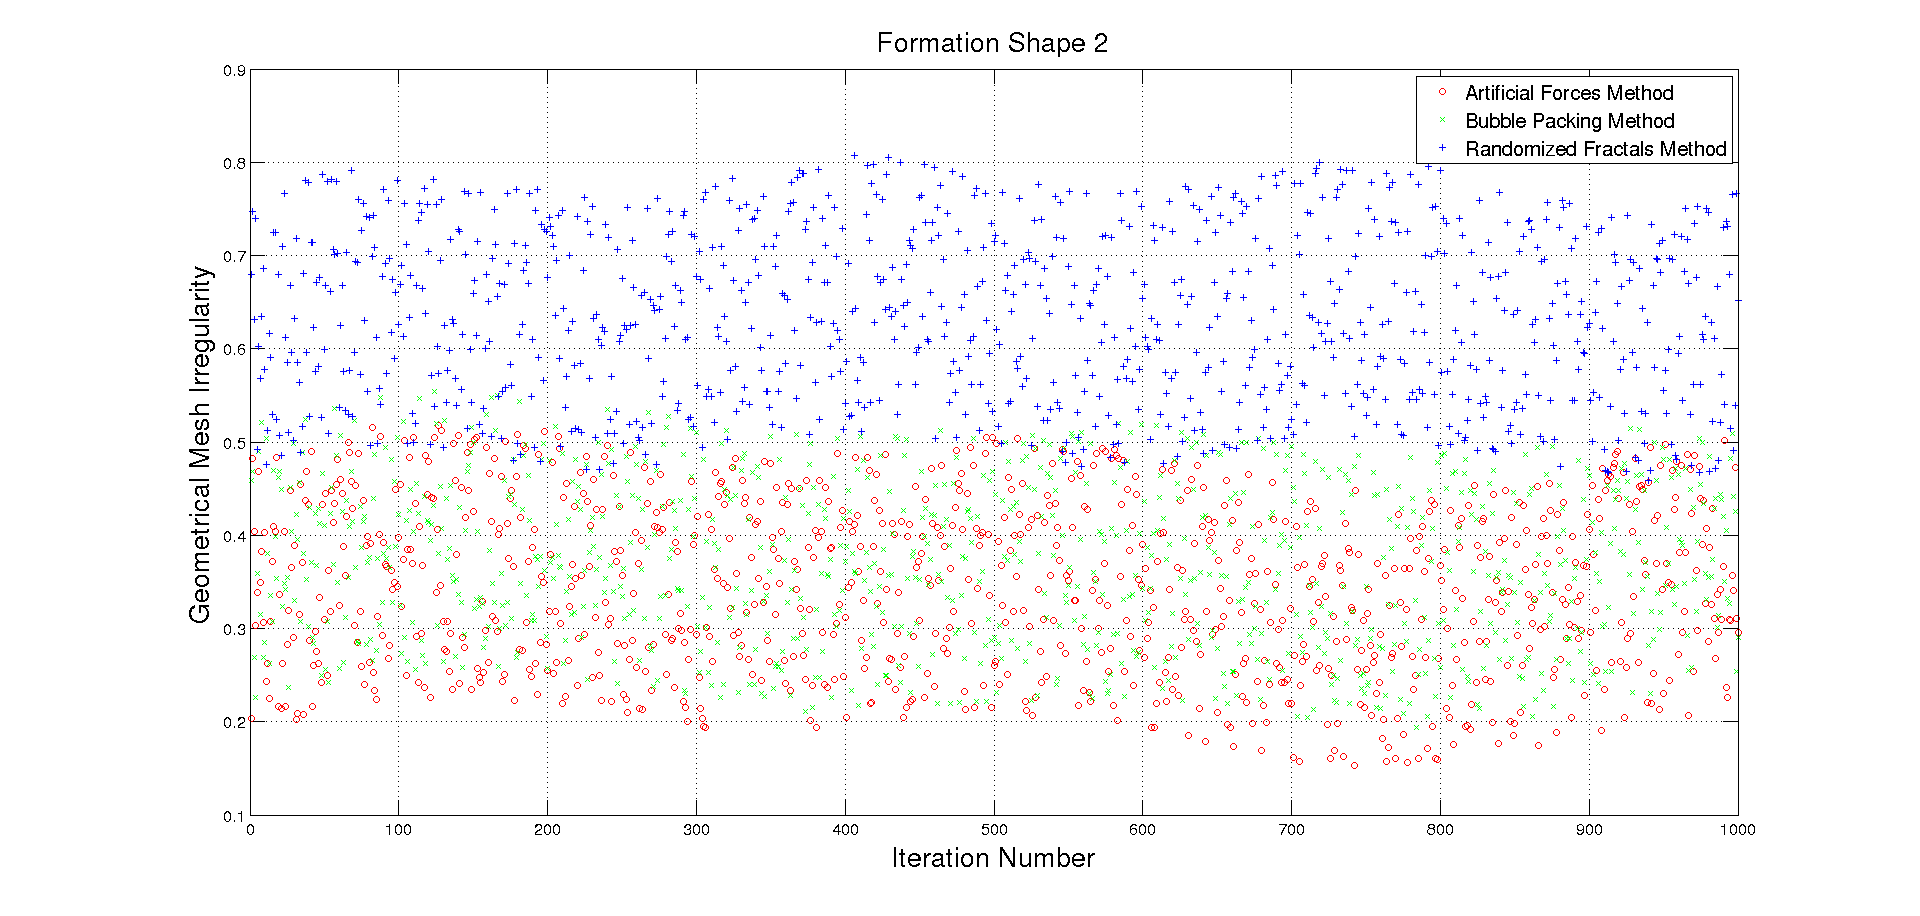
\includegraphics[scale = 0.45]{Geometrical_Irr_2}}
								\end{figure} 	
		
		
		
		
		  \subsubsection{Total Energy Consumption} 
		
		In this thesis work, it is aimed to minimize the overall energy consumption of the swarm while getting the desired formation shape. Here the energy consumption of the swarm is defined as the sum of the consumed energy by the individual agents. Monte Carlo simulations with 1000 iterations are handled for the same formations shapes with different same initial conditions of the agents in the environment. 				Trajectories of the agents are recorded from the same initial positions until the goal states for three different types of formation control systems. Total energy consumption of the swarm is measured with total position displacements of the agents while getting the desired formation shapes. Sample outputs for three different types of formation control algorithms are illustrated in the following Figures.
		
   \paragraph{Formation Shape 1}\hspace{0pt} \\
		
			\begin{figure}[H]
				\caption{Formation Shape 1 in MATLAB environment:}
				\centerline{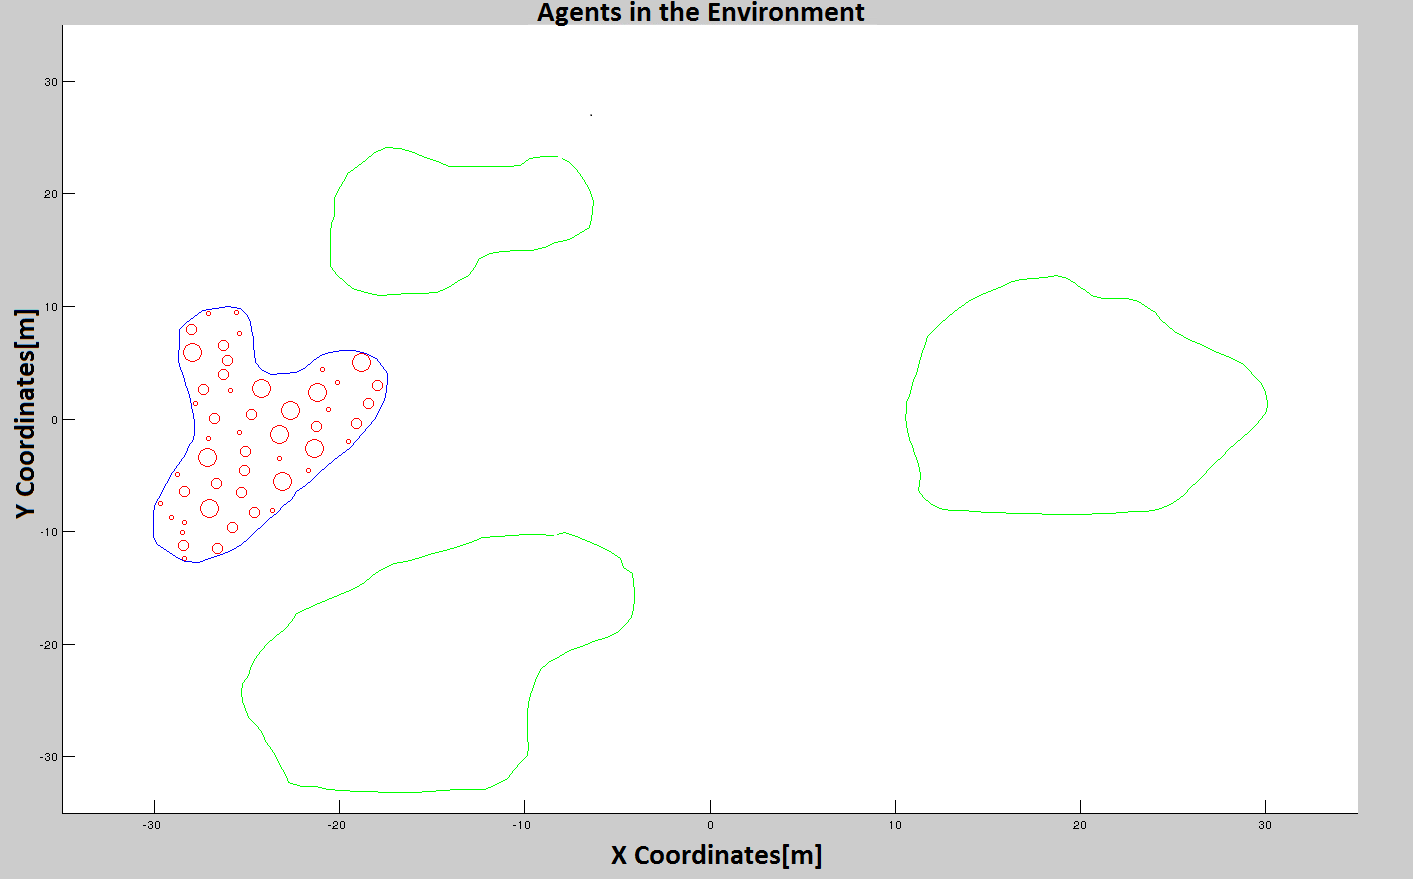
\includegraphics[scale = 0.40]{Trajectories_Formation_Shape_1_2}}
			\end{figure} 	
			
				\begin{figure}[H]
					\caption{Formation Shape 1 in Gazebo environment:}
					\centerline{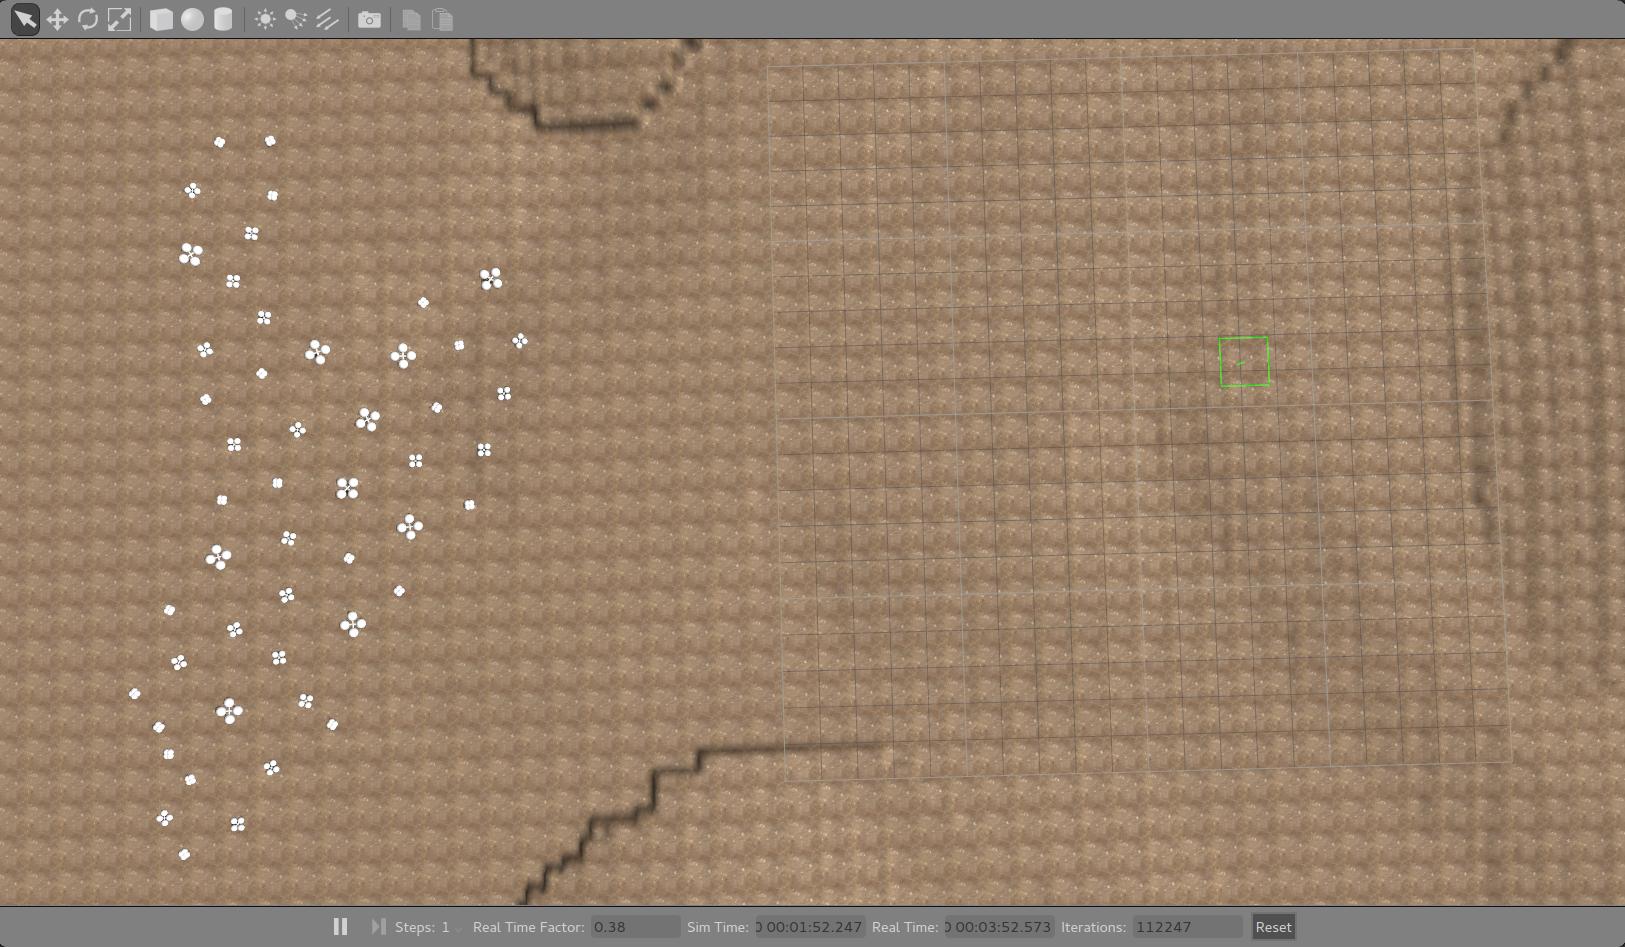
\includegraphics[scale = 0.35]{Trajectories_Formation_Shape_1_1}}
				\end{figure} 	
		
			\begin{figure}[H]
				\caption{Artificial Forces Method Trajectories for Shape 1}
				\centerline{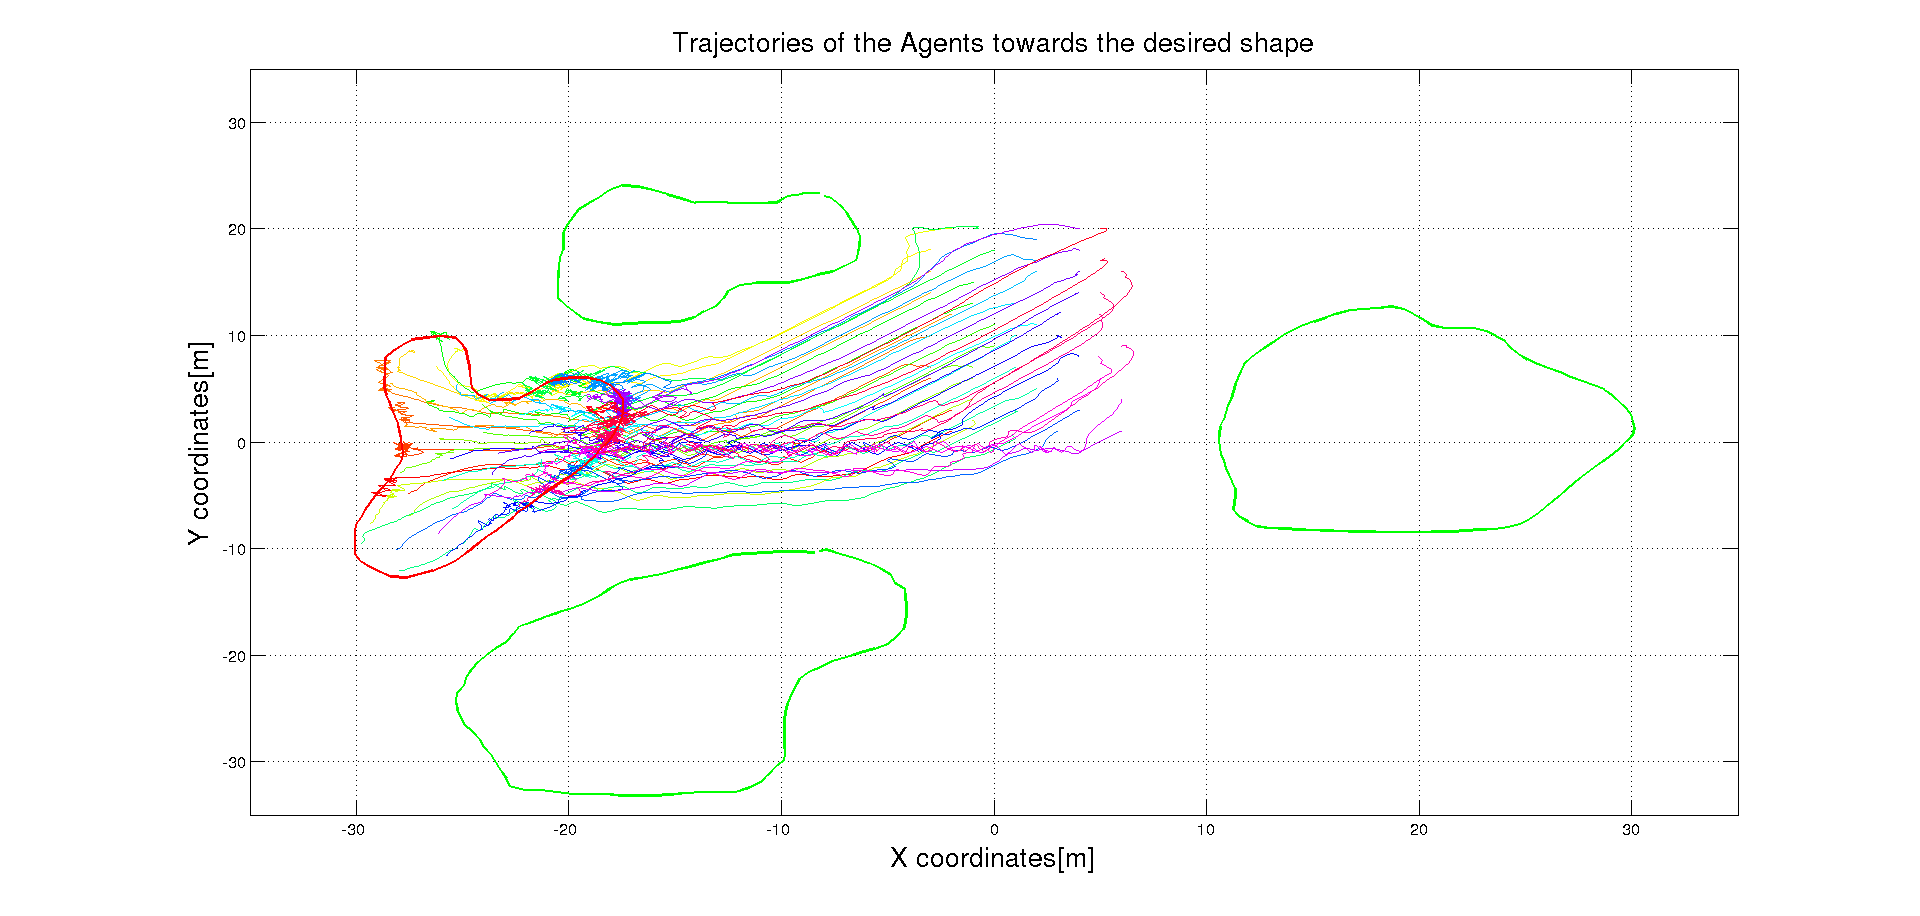
\includegraphics[scale = 0.35]{Aritificial_Trajecories_1}}
			\end{figure} 	

		\begin{figure}[H]
			\caption{Bubble Packing Method Trajectories for Shape 1}
			\centerline{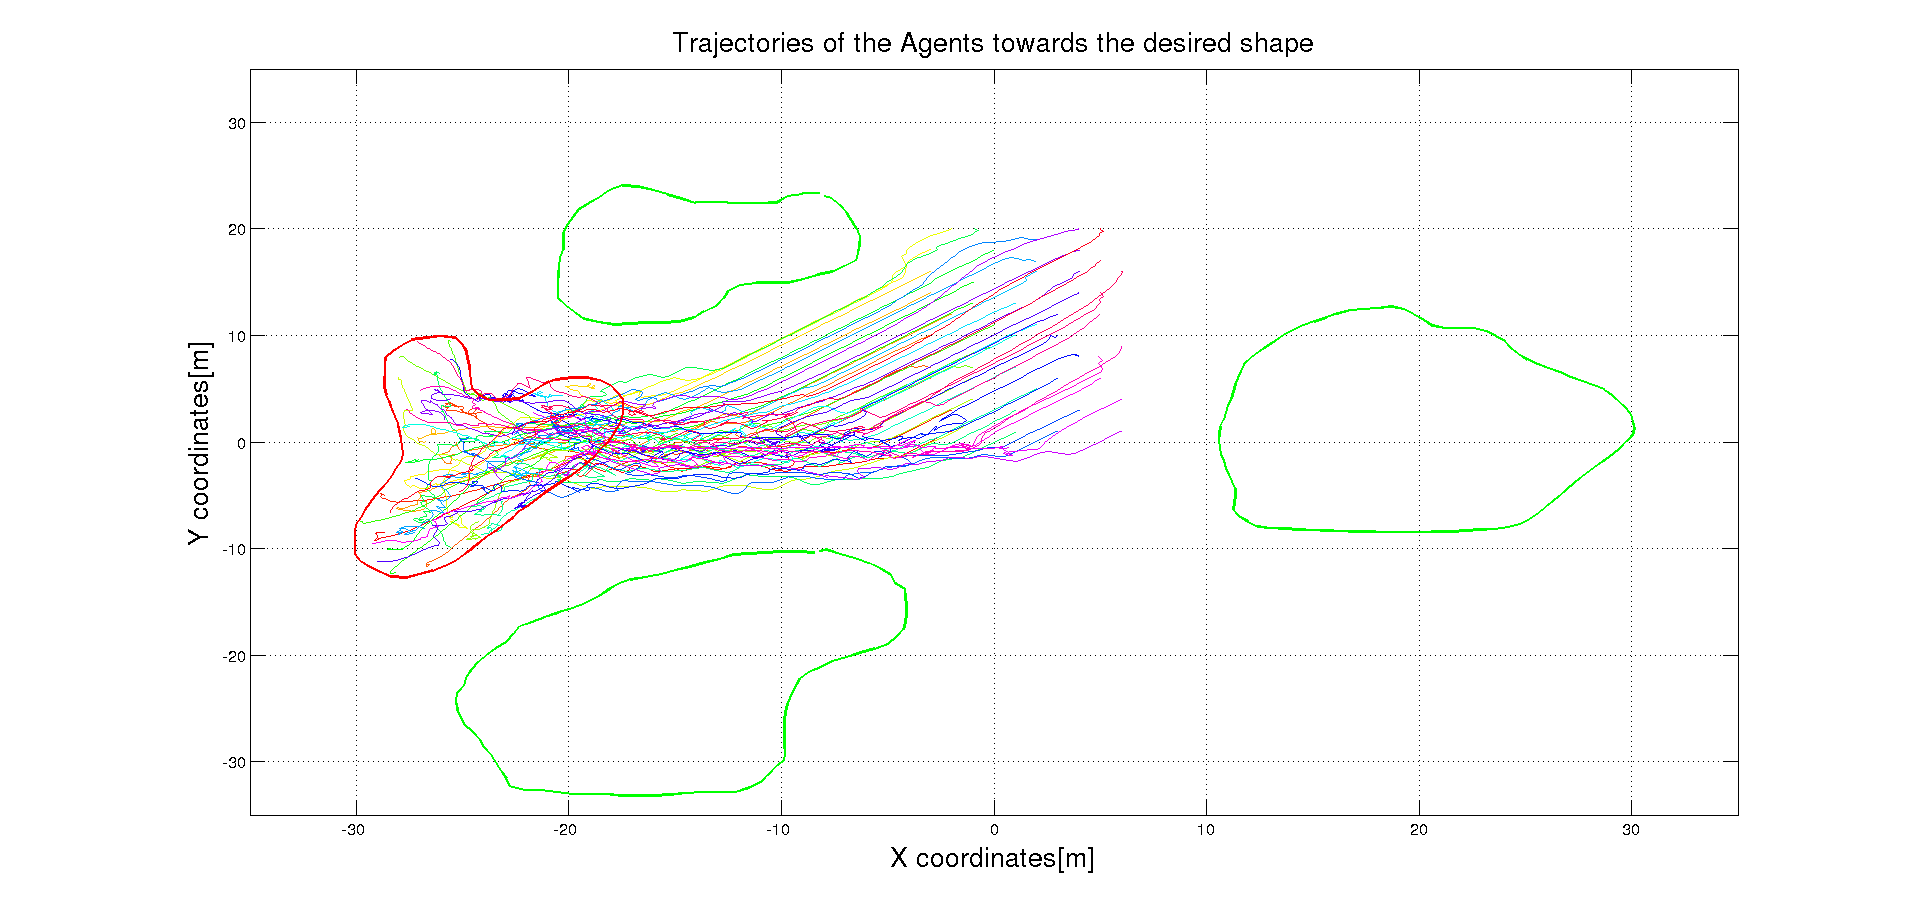
\includegraphics[scale = 0.35]{Bubble_Trajectories_1}}
		\end{figure} 	
		
			\begin{figure}[H]
				\caption{Randomized Fractals Method Trajectories for Shape 1}
				\centerline{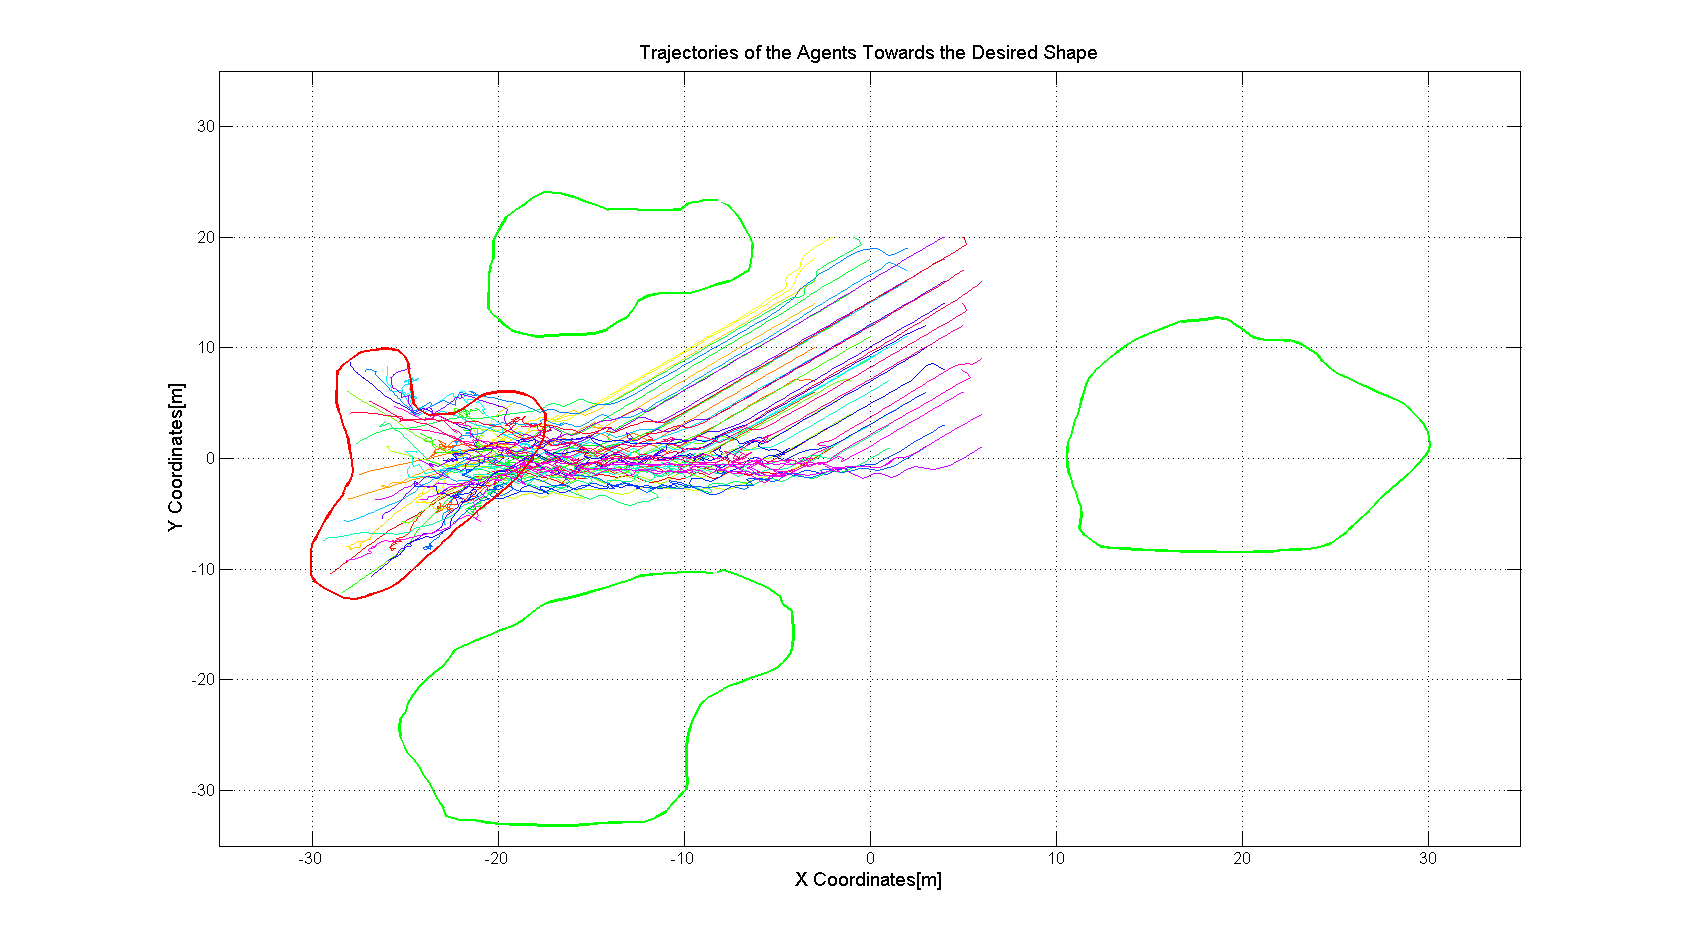
\includegraphics[scale = 0.35]{Randomized_Trajectories_1}}
			\end{figure} 	
			
		It is obvious that the trajectories of the agents are more chaotic and complex in the Artificial Forces method according to the other two solutions. This is because the agents are under the effect of a total force which is instantly changing both amplitude and direction with the local interactions in the environment. According to the X-Swarm theory which is described in Section-xx, all agents will move towards the center of the formation shape if the X Swarm conditions are satisfied by the agents. So the only force component which provides the distribution of the agents in the formation shape homogenously is the intermember forces which is dynamically changing so much with the local instant neighbors of the agents in the environment. On the other hand, Bubble Packing and Randomized Fractal methods implement an algorithm in which every agent is directed to a goal state in which the total energy consumption is minimized. This approach prevents the chaotic appearance of the trajectories and minimizes the energy consumption.
		Monte Carlo simulations with 1000 iterations are held and the results are presented in Figure -xx. 
		
		\begin{figure}[H]
			\caption{Total Energy Consumption}
			\centerline{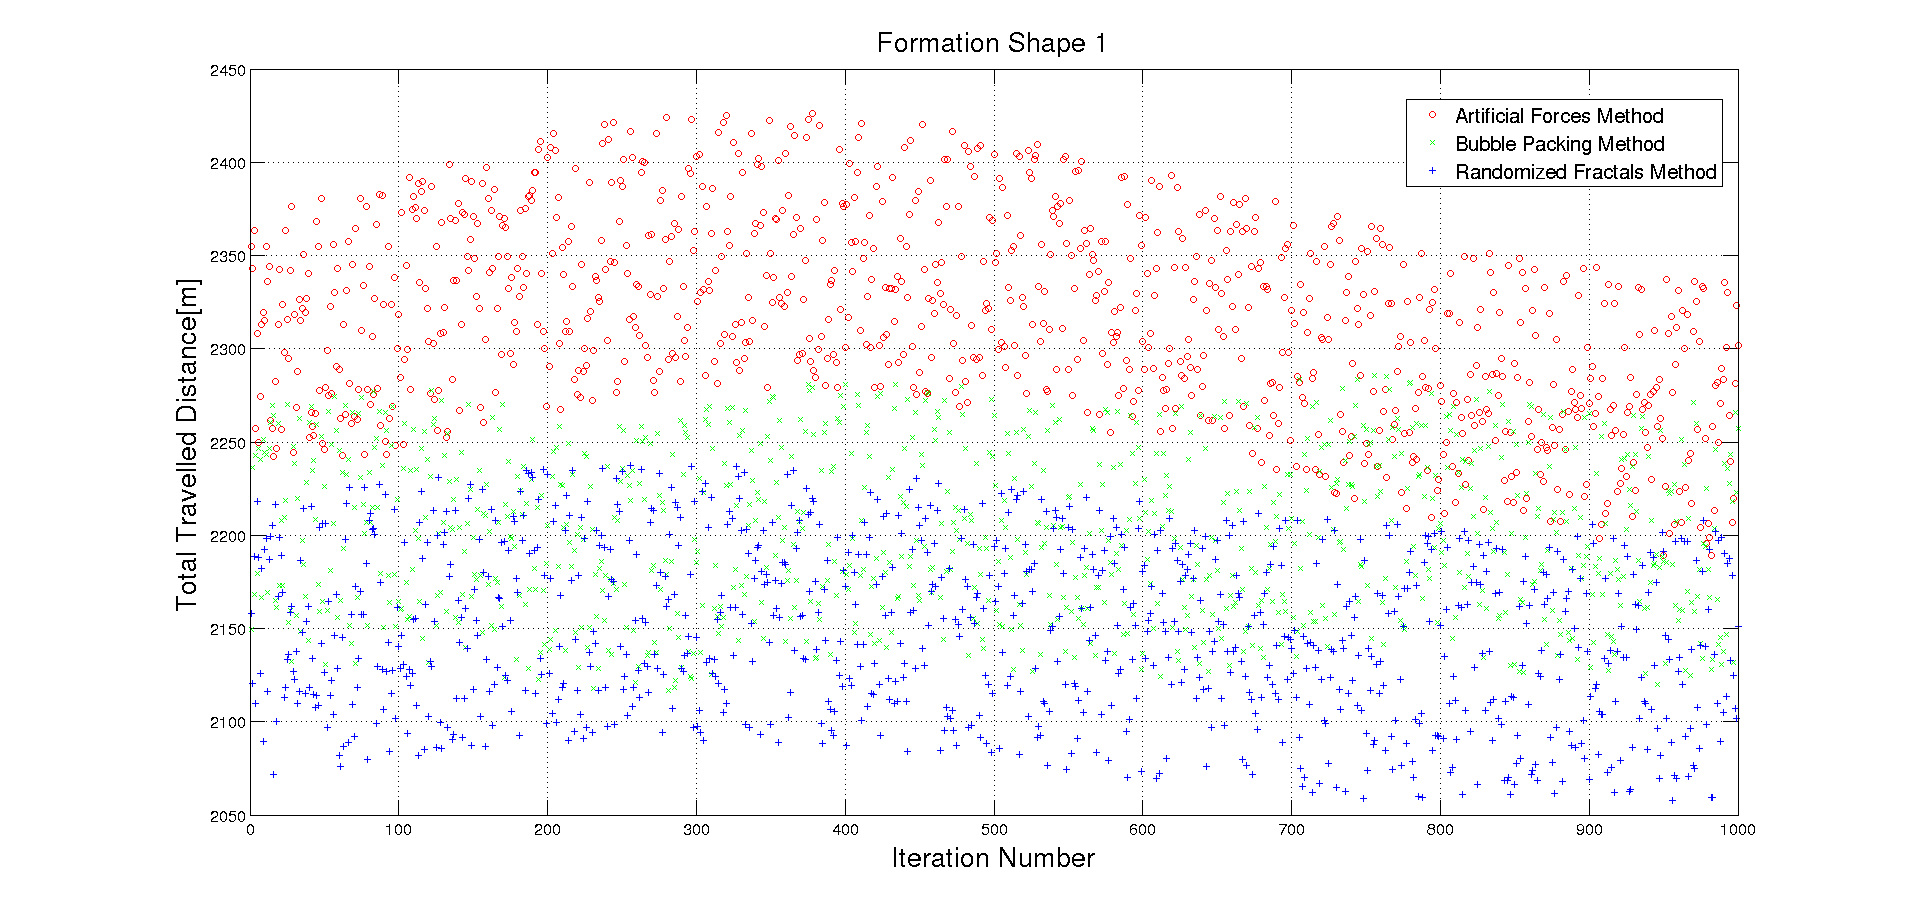
\includegraphics[scale = 0.35]{Total_Energy_Shape_1}}
		\end{figure} 	
		
		
		
		
		   \paragraph{Formation Shape 2}\hspace{0pt} \\
Second formation shape gives similar results with three different formation control methods, the Artificial Forces Method increases the total energy consumption of the agents because of the reasons discussed for the Formation Shape 1.

		   \begin{figure}[H]
		   	\caption{Formation Shape 2 in MATLAB environment:}
		   	\centerline{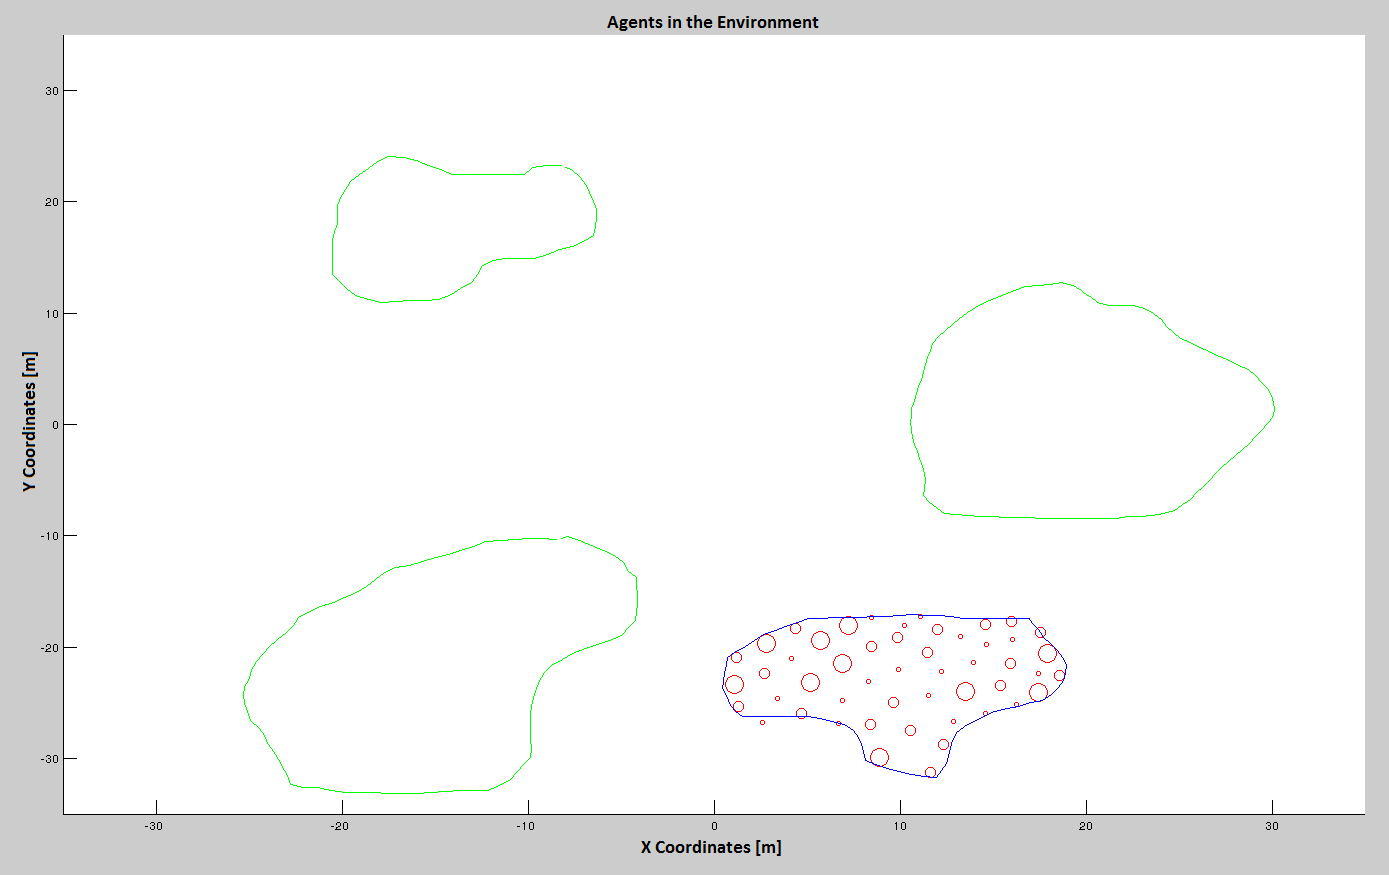
\includegraphics[scale = 0.40]{Trajectories_Formation_Shape_2_2}}
		   \end{figure} 	
		   
		   \begin{figure}[H]
		   	\caption{Formation Shape 2 in Gazebo environment:}
		   	\centerline{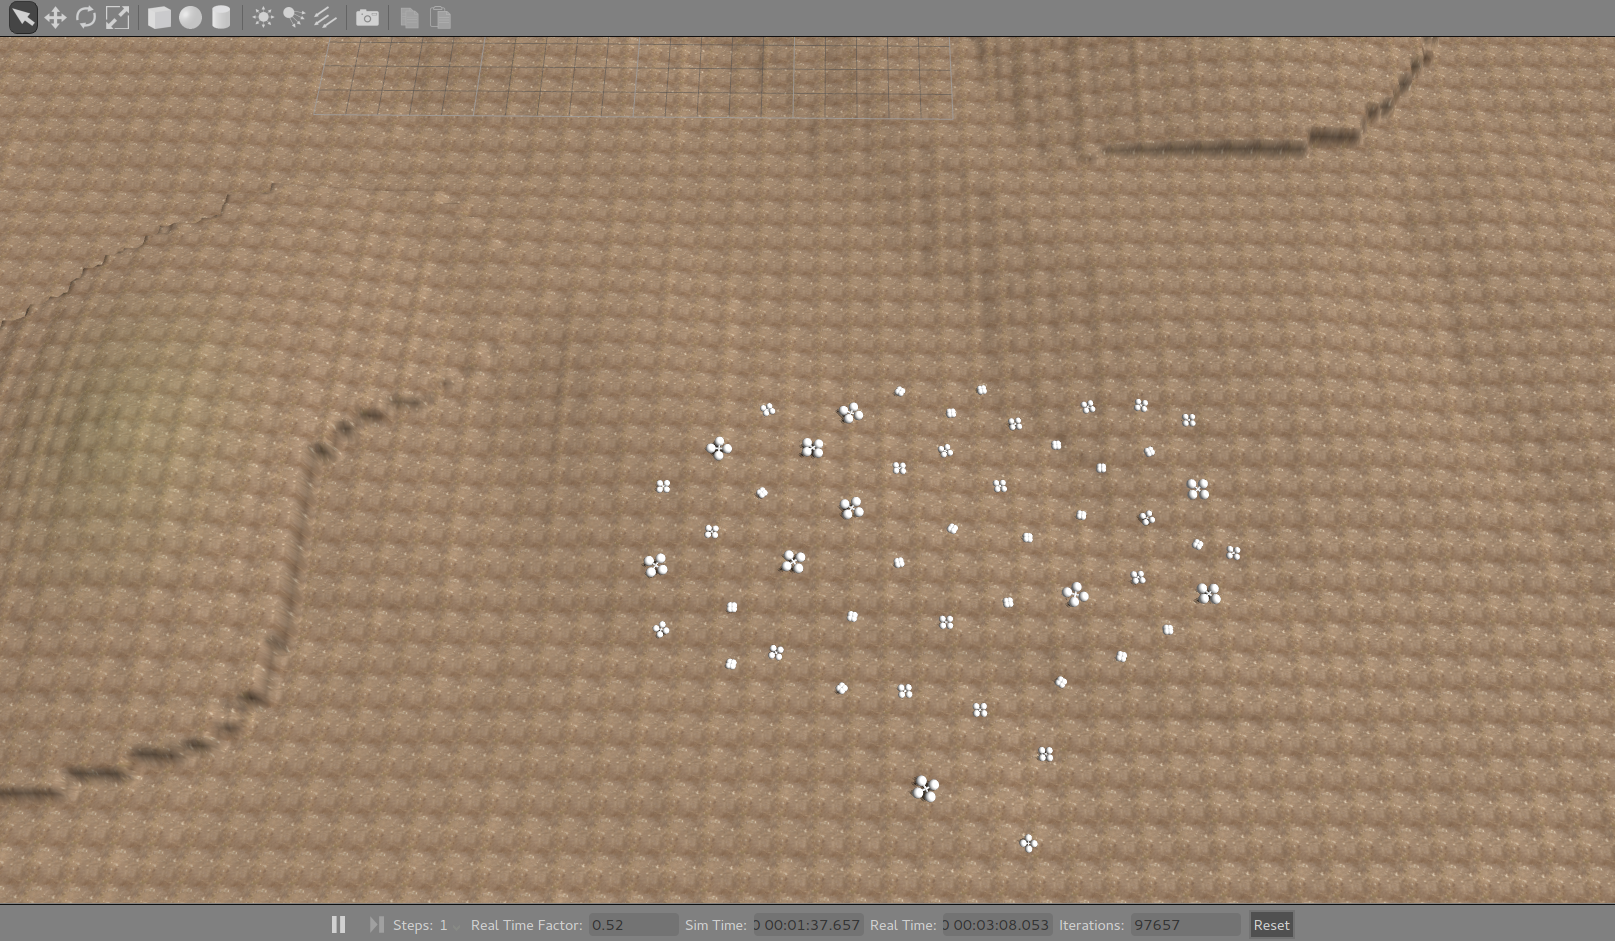
\includegraphics[scale = 0.35]{Trajectories_Formation_Shape_2_1}}
		   \end{figure} 	
		   
		   \begin{figure}[H]
		   	\caption{Artificial Forces Method Trajectories for Shape 2}
		   	\centerline{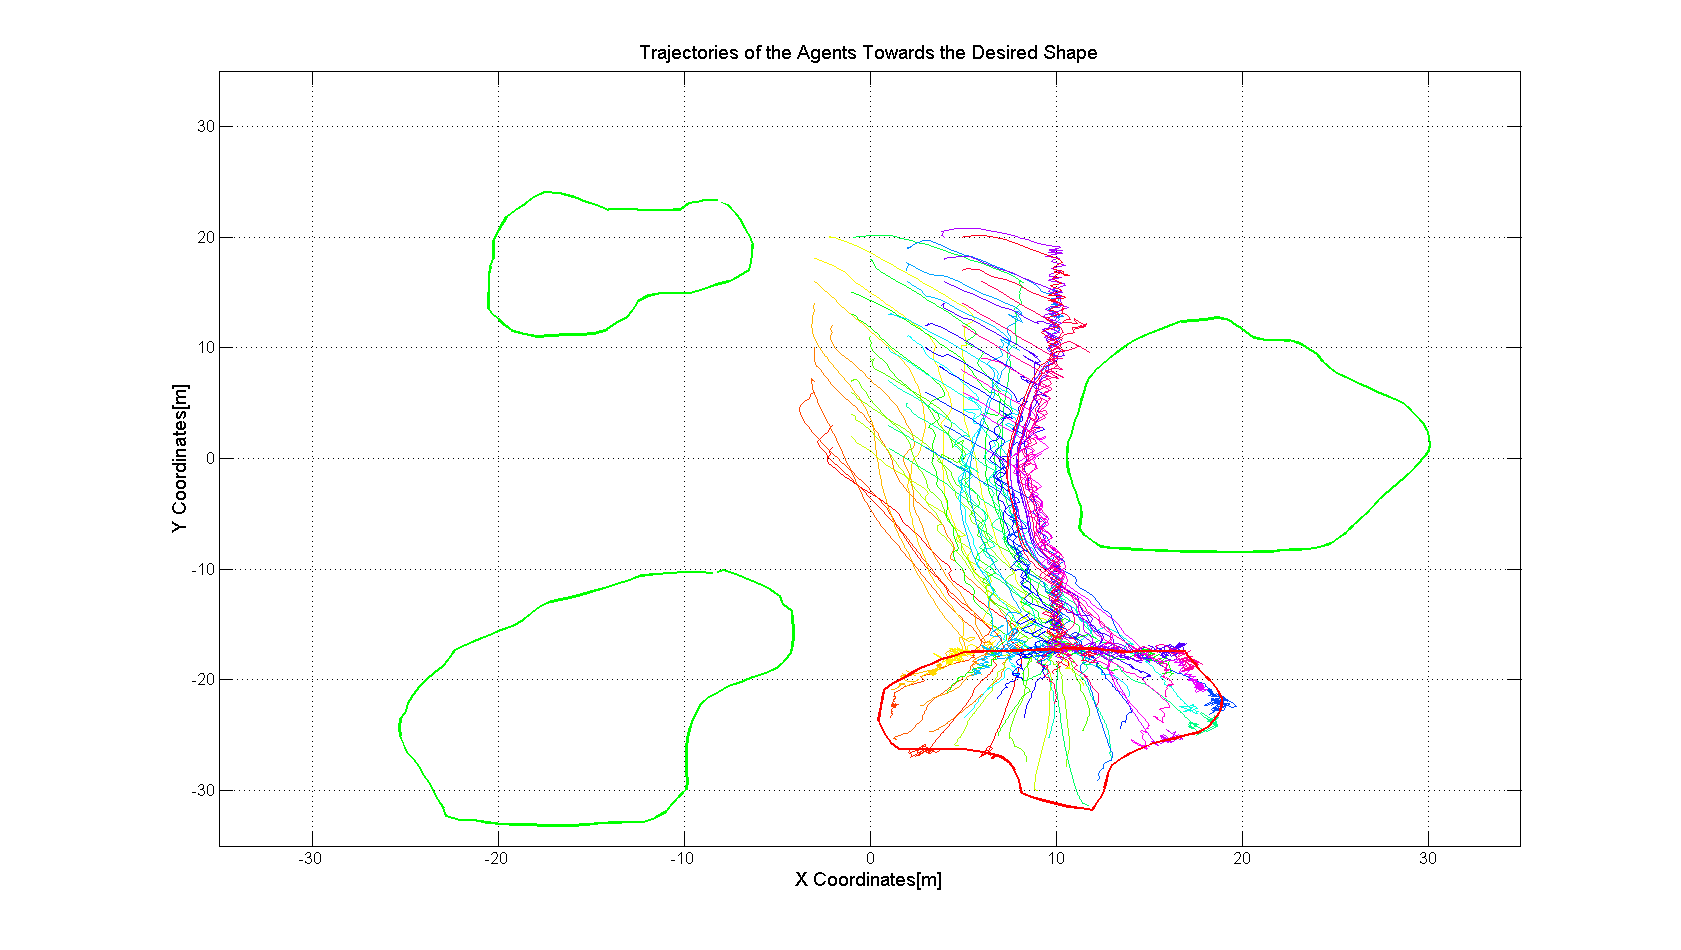
\includegraphics[scale = 0.35]{Artificial_Trajectories_2}}
		   \end{figure} 	
		   
		   \begin{figure}[H]
		   	\caption{Bubble Packing Method Trajectories for Shape 2}
		   	\centerline{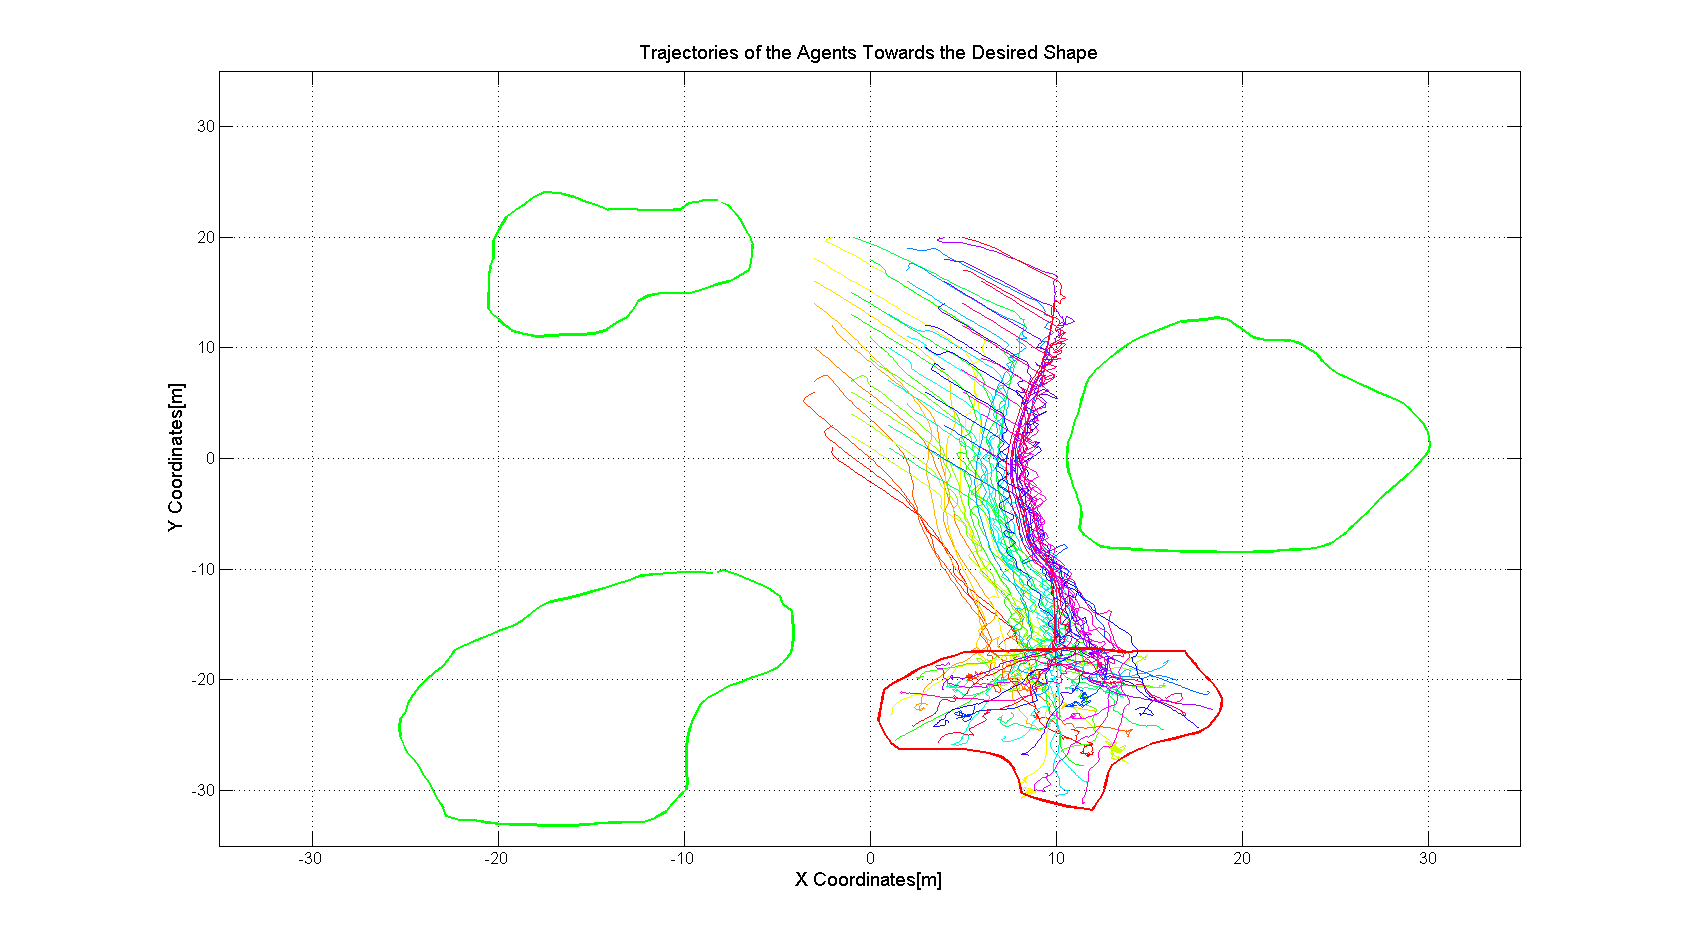
\includegraphics[scale = 0.35]{Bubble_Trajectories_2}}
		   \end{figure} 	
		   
		   \begin{figure}[H]
		   	\caption{Randomized Fractals Method Trajectories for Shape 2}
		   	\centerline{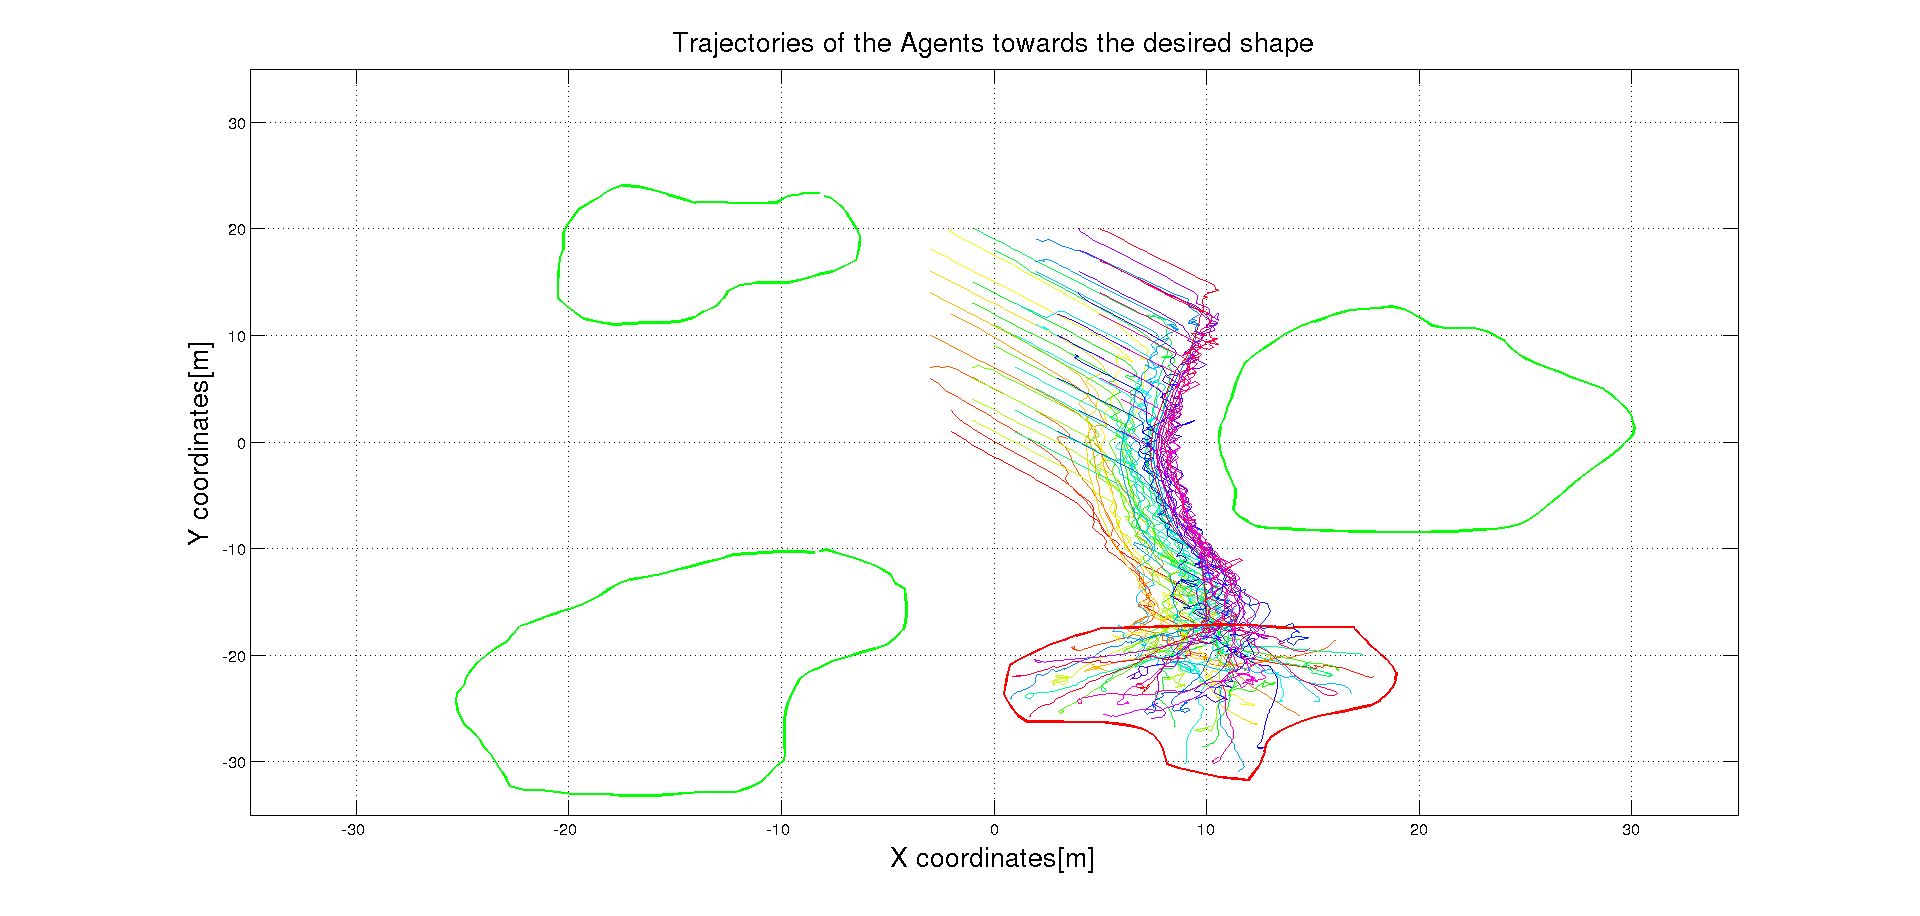
\includegraphics[scale = 0.35]{Randomized_Trajectories_2}}
		   \end{figure} 	
		   
        The results of the Monte Carlo simulations with 1000 iterations are illustrated in Figure -xx /
		   \begin{figure}[H]
		   	\caption{Total Energy Consumption}
		   	\centerline{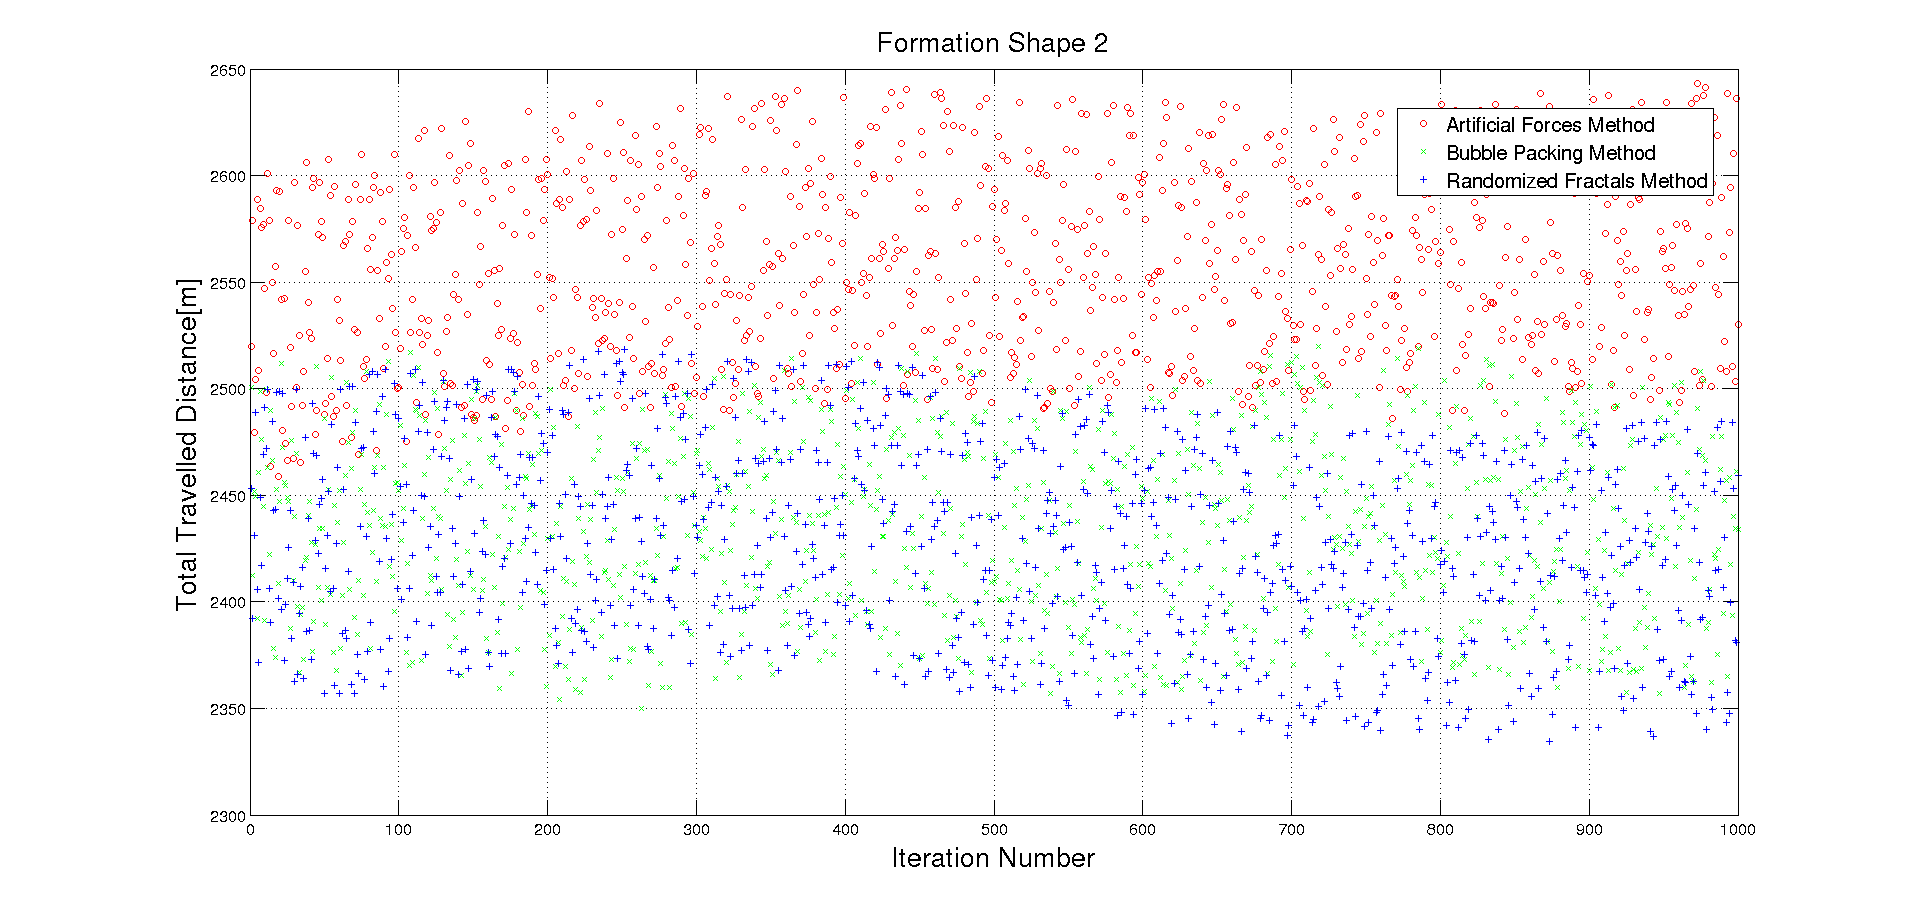
\includegraphics[scale = 0.35]{Total_Energy_Shape_2}}
		   \end{figure} 	
		   
		
		
		
		  \subsubsection{Settling Time} 
		
		Settling time is defined as delta time $"t_{final} - t_{start}"$ ,where $t_{start}$ is the initial time and $t_{final}$ is the time that the all of the agents are inside of the desired formation shape and the norm of the velocity vector for each agent $\norm{v_i}$ is
		
		\begin{equation}
\norm{v_i(t)} < 0.01 \hspace{0.1cm} [m/sec] \hspace{0.3cm}\forall\hspace{0.05cm} t>t_{final}
		\end{equation}
		
		Settling times are measured for the simulations held in Energy Consumption Part-xx, and Artificial Forces method have the worst performance as expected. Since there are no predetermined goal states for the agents in the desired formation shape, the settling of the agents in random places under the equilibrium of the artificial force components takes much more time than the other two formation control methods. The agents have reached the steady state at their goal states with the shape partitioning methods faster than the Artificial Forces Methods. The results are illustrated in Figure-xx.
		
		   \begin{figure}[H]
		   	\caption{Total Settling Time for Shape 1}
		   	\centerline{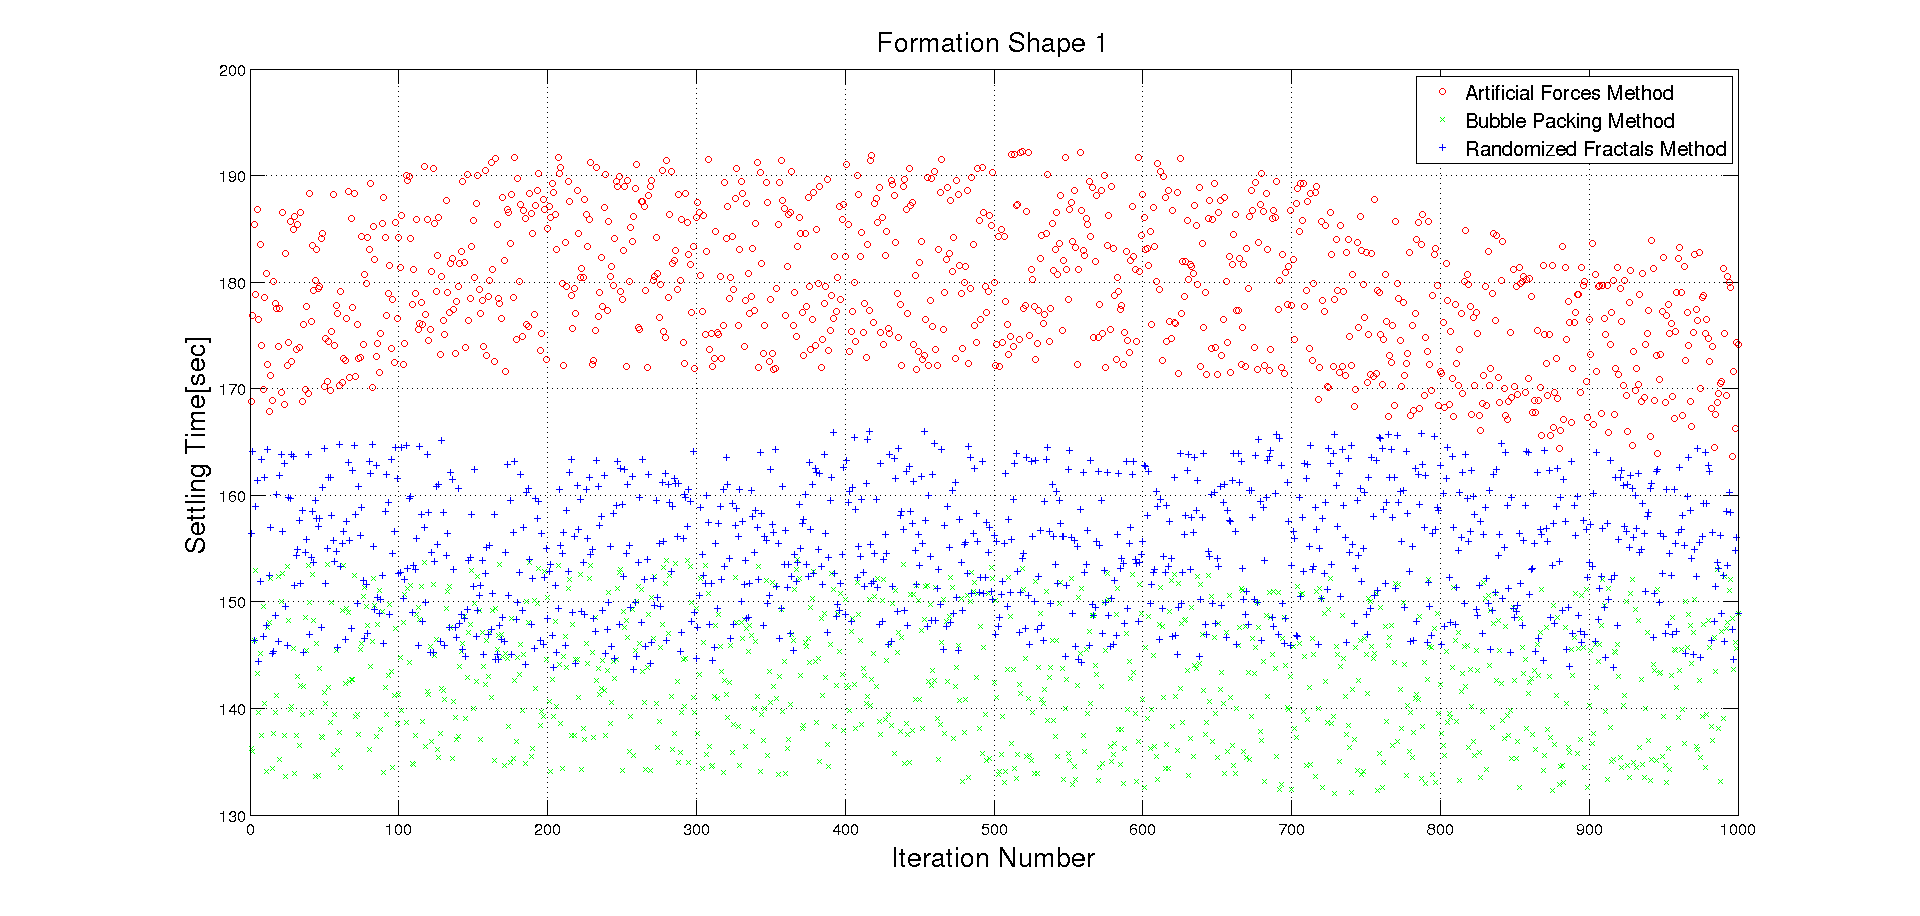
\includegraphics[scale = 0.35]{Total_Time_Shape_1}}
		   \end{figure} 
		
		 \begin{figure}[H]
		 	\caption{Total Settling Time for Shape 2}
		 	\centerline{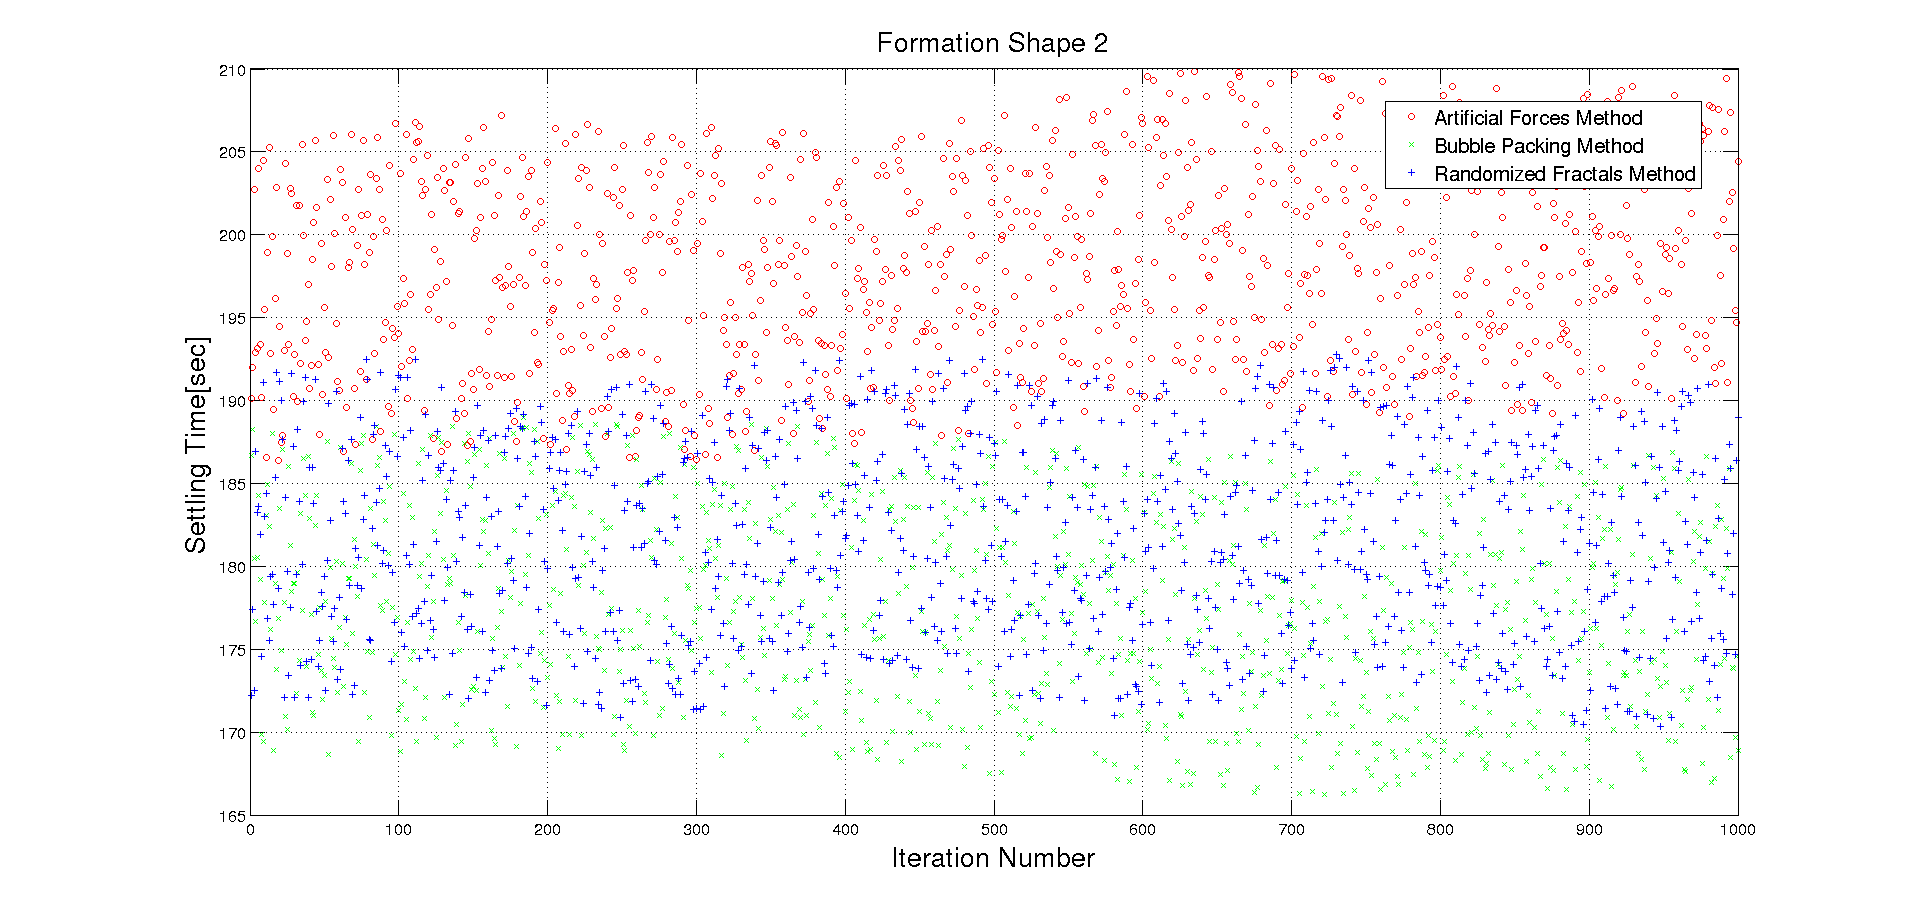
\includegraphics[scale = 0.35]{Total_Time_Shape_2}}
		 \end{figure} 
		 
		 
		
			 \subsubsection{Evaluation} 
		Three different formation control approaches are evaluated with different kinds of metrics including the total energy consumption, settling time and mesh quality which is a measure of how the agents homogenously distributed while covering the desired formation shape. Artificial forces method have the worst performance in setlling time and energy consumption metrics due to the absence of predetermined goal states which is discussed in Section-xx in details. On the other hand the Randomized Fractals method have the worst mesh quality performance because of its randomized nature of assignment the goal states in the desired formation shape. The methods which have the worst performance at the related metrics are illustrated in Table -xx
		
		
		\begin{center}
			\captionof{table}{Formation Control Methods with Worst Performance} \label{tab:title} 
			\begin{tabular}{||c| c| c |c ||}
				
				\hline
				\textbf{Method/Metric} & \textbf{Energy Consumption}  & \textbf{Settling Time} & \textbf{Mesh Quality}\\ 
				\hline
				Artificial Force & X & X &  \\
				Bubble Packing & &  &  \\	
				Randomized Fractals & &  & X \\	
				\hline
			\end{tabular}
		\end{center}
		
		It is obvious that time Bubble Packing Method have the best performance for all metrics. In fact, Bubble Packing method combines the efficient approaches of the other two methods. In the shape partitioning phase of the algorithm, it uses interbubble forces which have a similar structure to the intermember forces applied by the Artificial Forces method in real time. This force have the greatest  effect on the homogeneity of the agents in the desired formation shape because it provides a global consensus for the agents in which each agent reaches an equilibrium state under the total forces acting by their neighbors and the formation shape. On the other hand, bubble packing method implements an algorithm in which every agent assigned to a goal state instantly at each execution time of the algorithm to minimize the overall energy consumption o the swarm. This approach reduce the settling time and the total displacements of the agents from the initial state to their final states since their final positions in the formation shape is predetermined. It is possible that the agents' goal states may be changed with the execution of the algorithm at different steps, but these assignments will converge to a uniqe subset while the agents are getting closer to the goal states. 
		
Some other formation shape trials with the Bubble Packing algorithm is illustrated in the follwoing Figures-xx.


		
		 \begin{figure}[H]
		 	\caption{Formation Shape - 1 in Gazebo Environment}
		 	\centerline{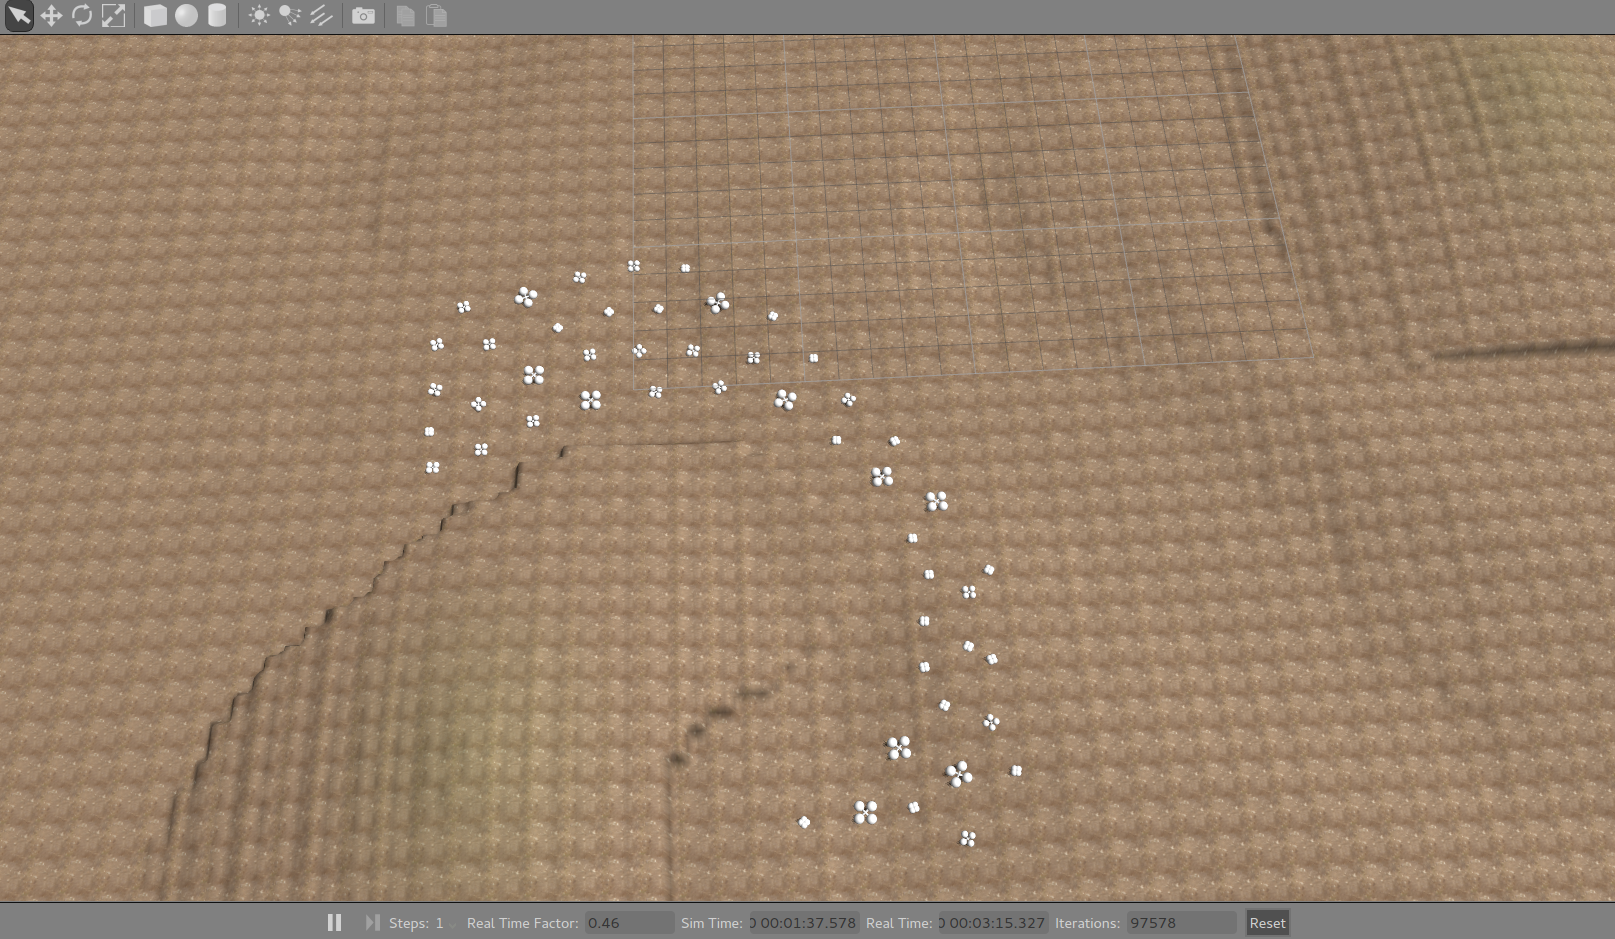
\includegraphics[scale = 0.35]{1_Gazebo}}
		 \end{figure} 
			
			\begin{figure}[H]
		 	\caption{Formation Shape - 1 in MATLAB Environment}
				\centerline{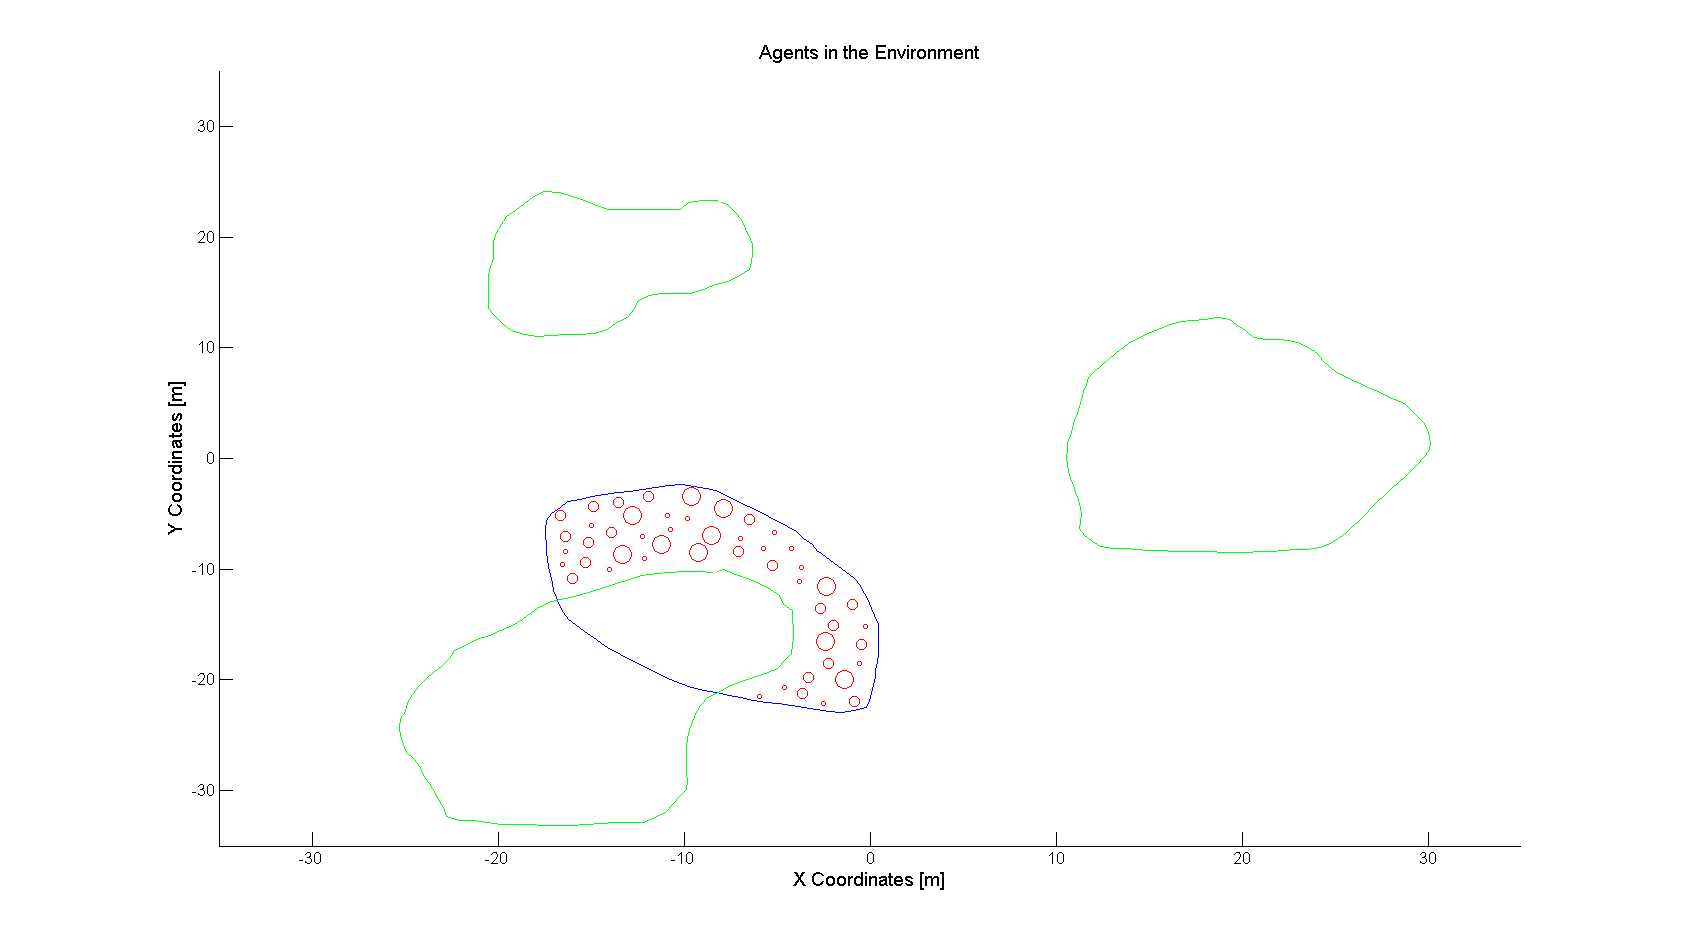
\includegraphics[scale = 0.40]{1}}
			\end{figure} 
			
			\begin{center}
				\captionof{table}{Performance Metrics for Shape - 1} \label{tab:title} 
				\begin{tabular}{||c| c |c |c ||}
					
					\hline
				 		\textbf{Energy Consumption[m]}  & \textbf{Settling Time[sec]} & \textbf{Topological Mesh Irregularity} & \textbf{Geometrical Mesh Irregularity}\\ 
					\hline
				 1889 & 164 &  2.54& 0.62\\
					\hline
				\end{tabular}
			\end{center}
		
		
		
		 \begin{figure}[H]
		 	\caption{Formation Shape - 2 in Gazebo Environment}
		 	\centerline{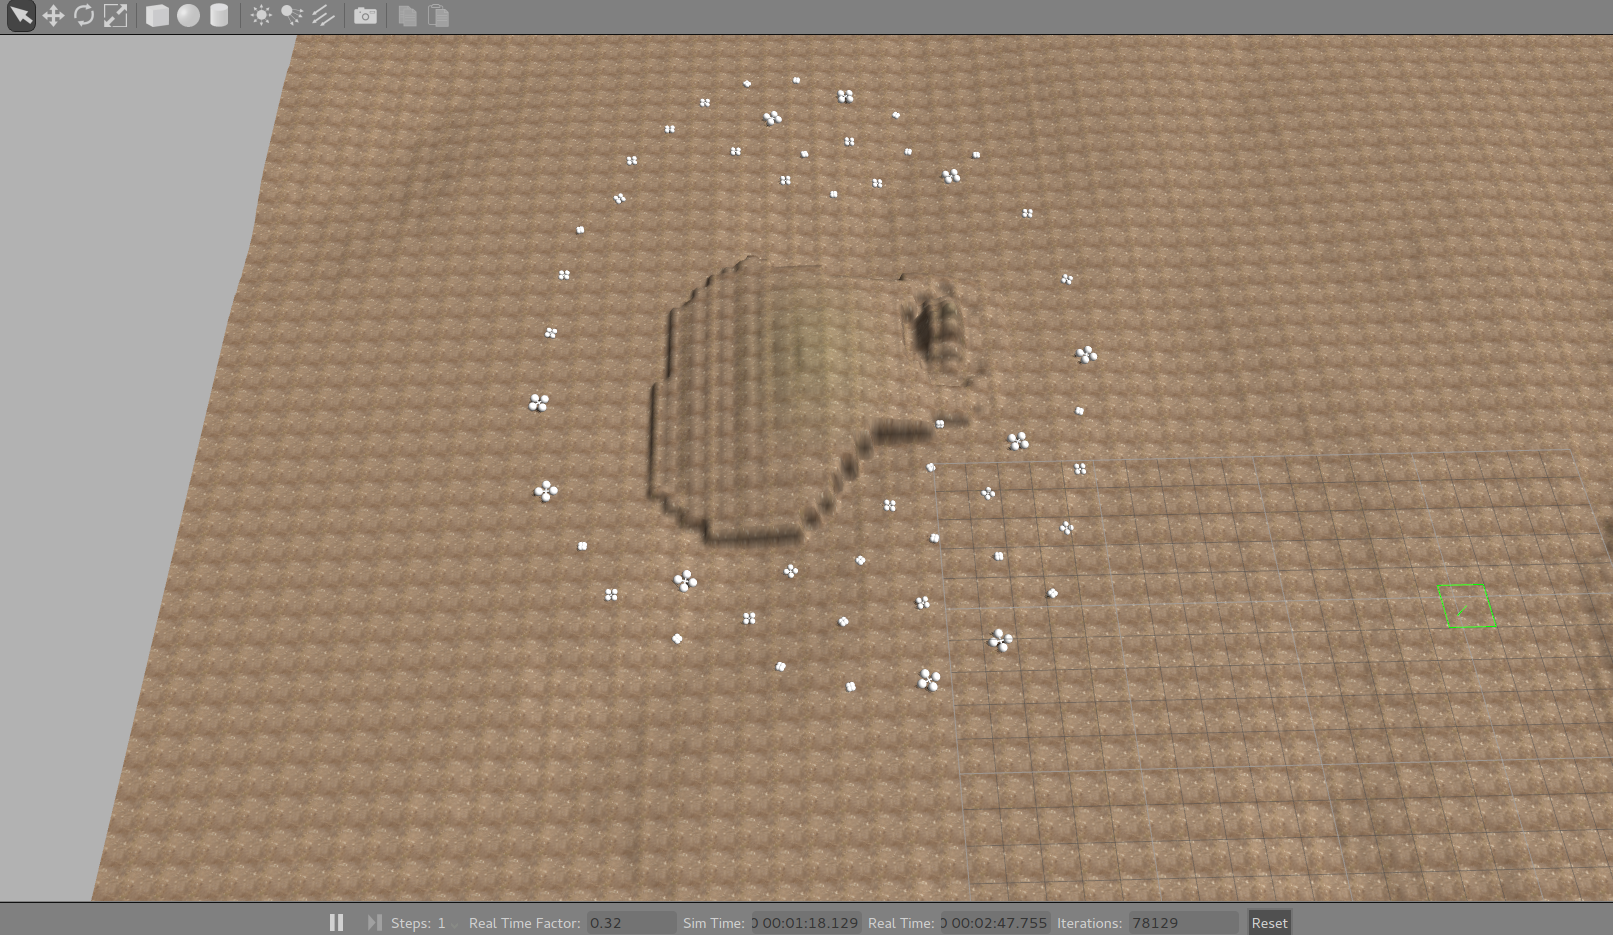
\includegraphics[scale = 0.35]{2_Gazebo}}
		 \end{figure} 
		 
		 \begin{figure}[H]
		 	\caption{Formation Shape - 2 in MATLAB Environment}
		 	\centerline{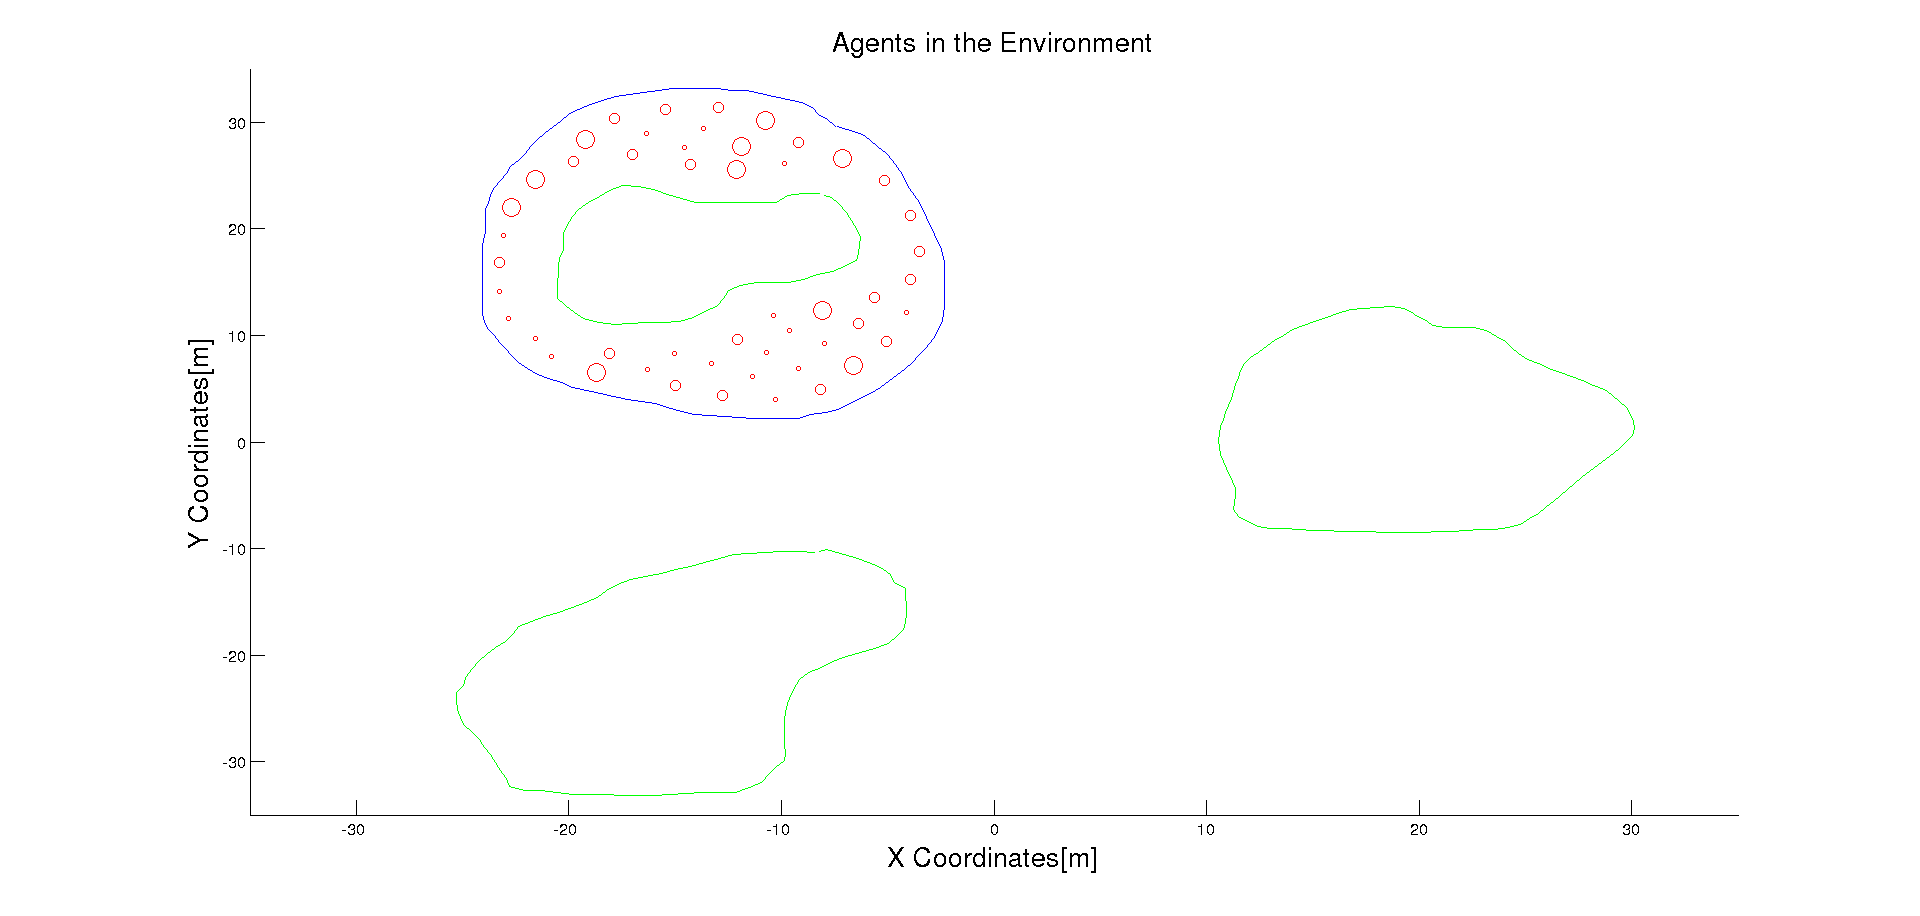
\includegraphics[scale = 0.40]{2}}
		 \end{figure} 
		 
		 \begin{center}
		 	\captionof{table}{Performance Metrics for Shape - 2} \label{tab:title} 
		 	\begin{tabular}{||c| c |c |c ||}
		 		
		 		\hline
				 		\textbf{Energy Consumption[m]}  & \textbf{Settling Time[sec]} & \textbf{Topological Mesh Irregularity} & \textbf{Geometrical Mesh Irregularity}\\ 
		 		\hline
		 		1611 & 153 &  2.95& 0.73\\
		 		\hline
		 	\end{tabular}
		 \end{center}
		 
		
		
				 \begin{figure}[H]
				 	\caption{Formation Shape - 3 in Gazebo Environment}
				 	\centerline{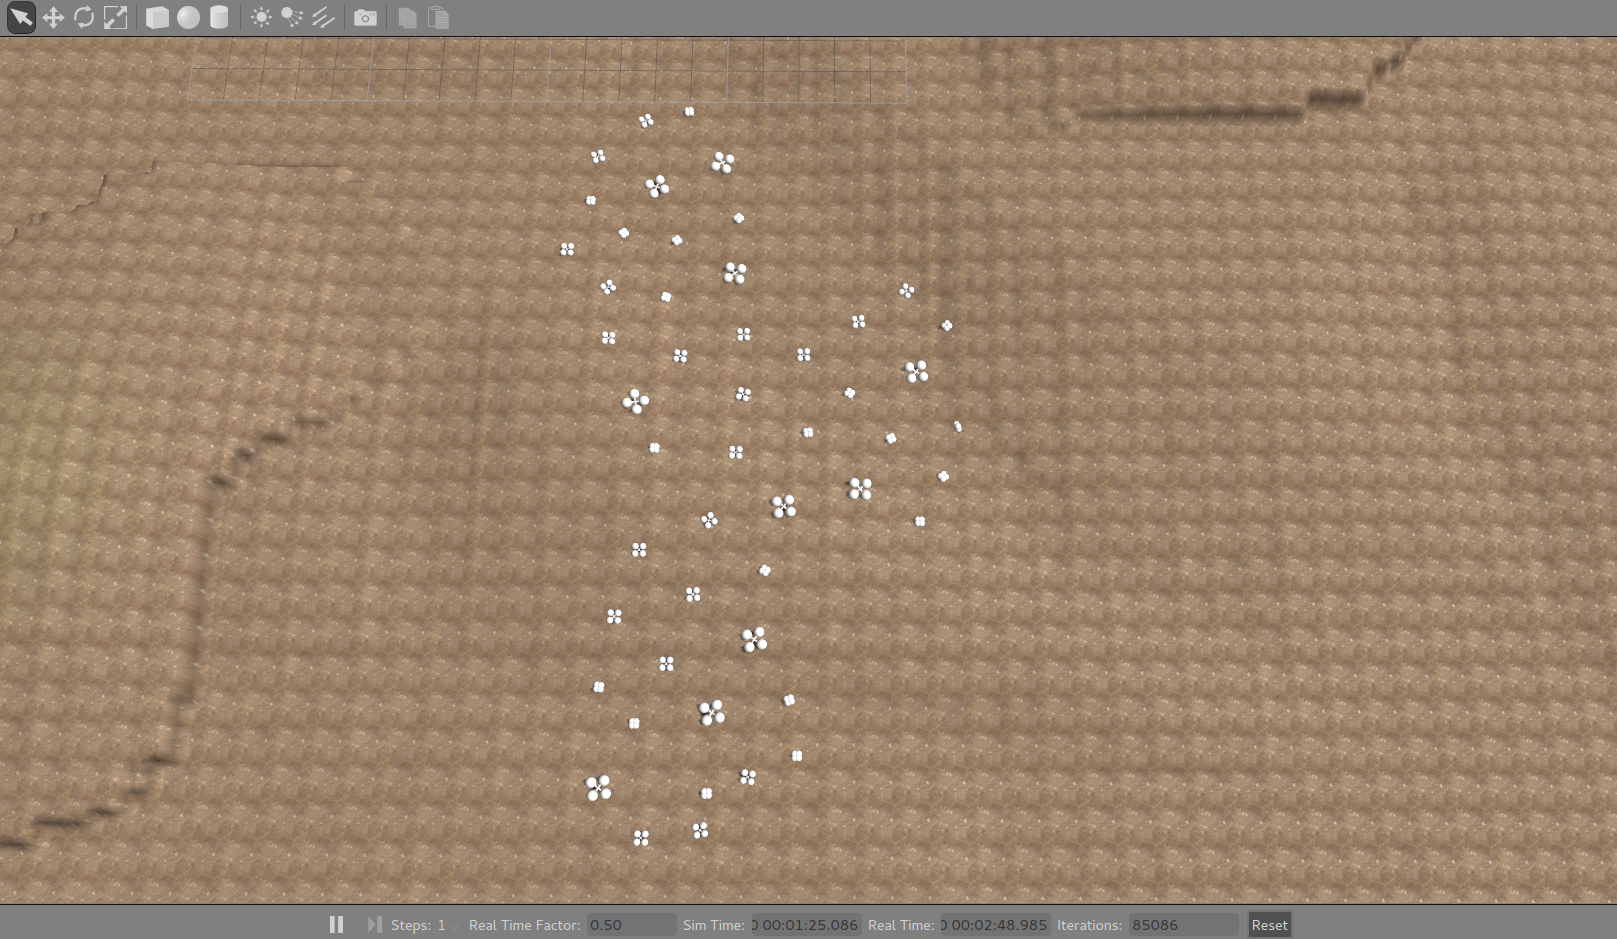
\includegraphics[scale = 0.35]{3_Gazebo}}
				 \end{figure} 
				 
				 \begin{figure}[H]
				 	\caption{Formation Shape - 3 in MATLAB Environment}
				 	\centerline{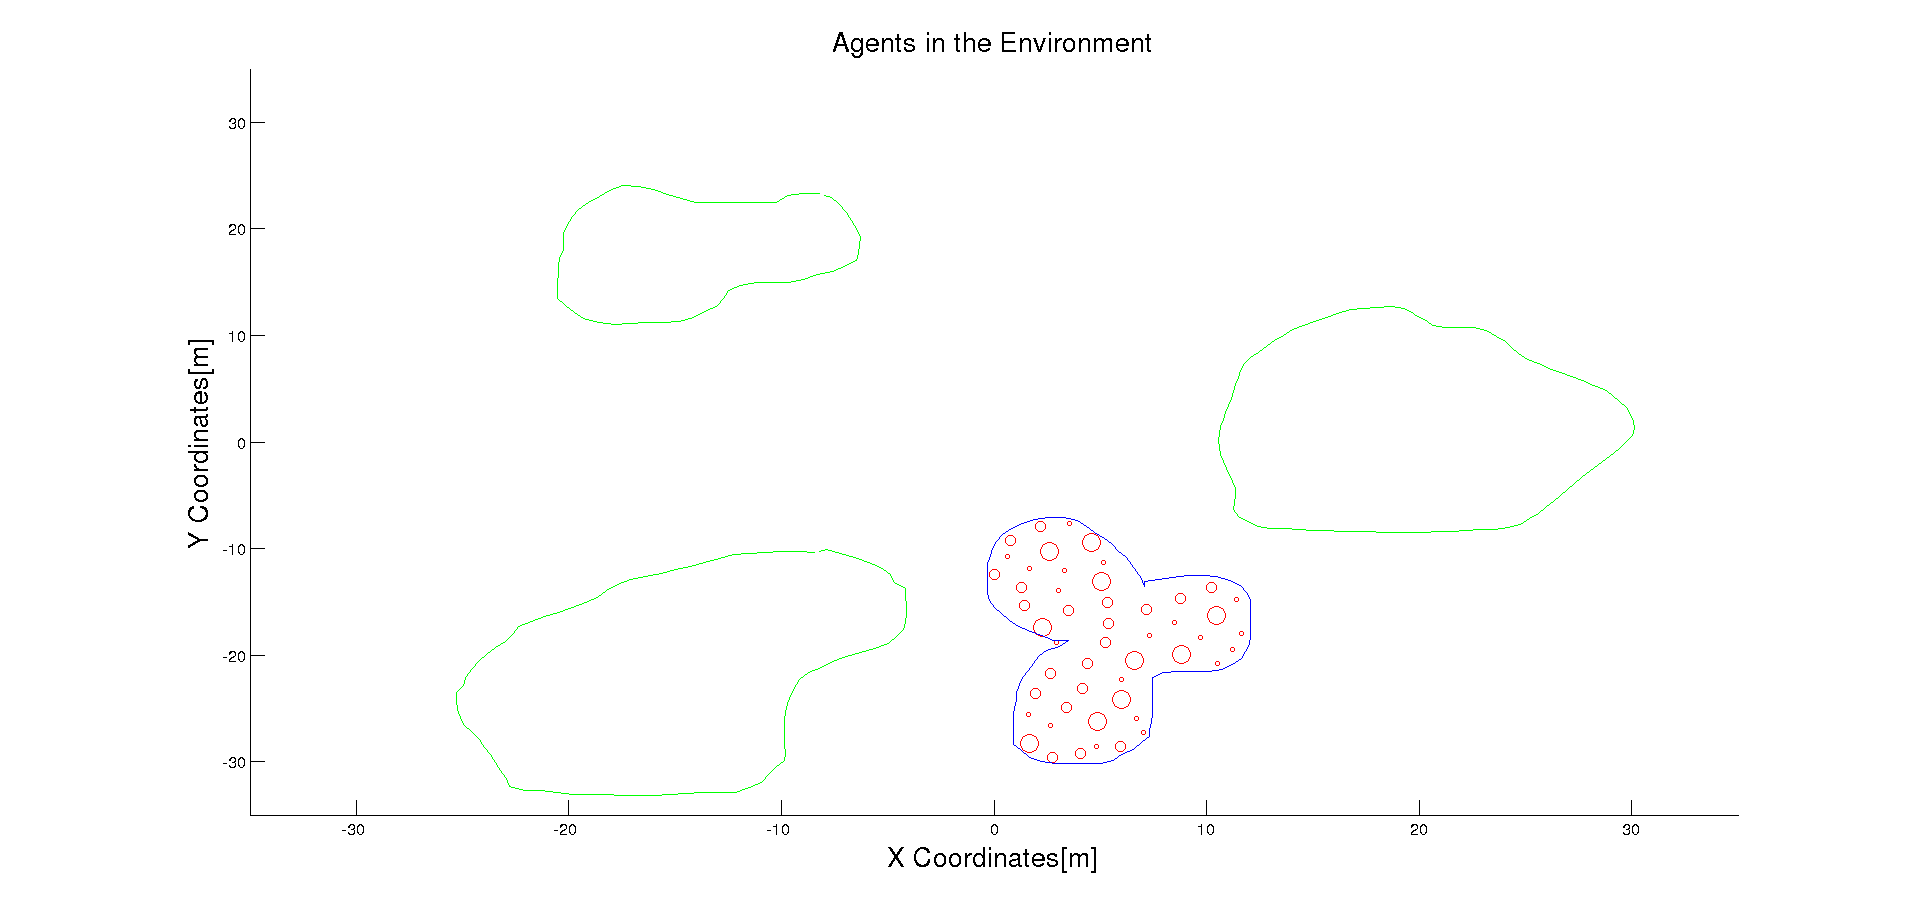
\includegraphics[scale = 0.40]{3}}
				 \end{figure} 
				 
				 \begin{center}
				 	\captionof{table}{Performance Metrics for Shape - 3} \label{tab:title} 
				 	\begin{tabular}{||c| c |c |c ||}
				 		
				 		\hline
				 		\textbf{Energy Consumption[m]}  & \textbf{Settling Time[sec]} & \textbf{Topological Mesh Irregularity} & \textbf{Geometrical Mesh Irregularity}\\ 
				 		\hline
				 		1432 & 126 &  2.23& 0.45\\
				 		\hline
				 	\end{tabular}
				 \end{center}
				 
				 
			
			\begin{figure}[H]
				\caption{Formation Shape - 4 in Gazebo Environment}
				\centerline{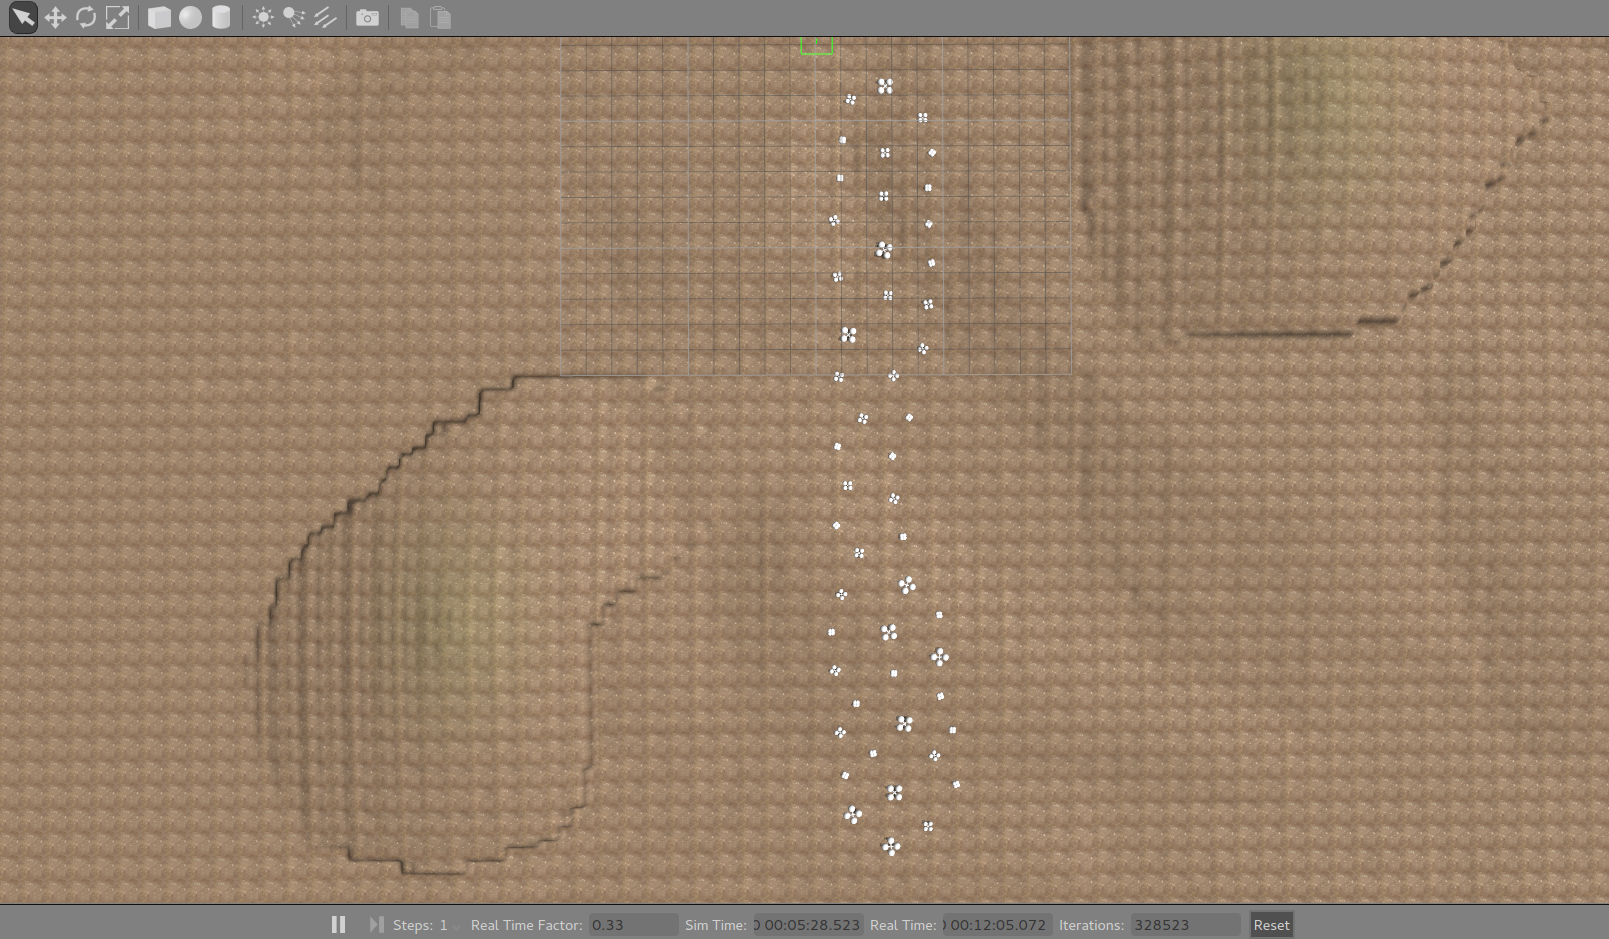
\includegraphics[scale = 0.35]{4_Gazebo}}
			\end{figure} 
			
			\begin{figure}[H]
				\caption{Formation Shape - 4 in MATLAB Environment}
				\centerline{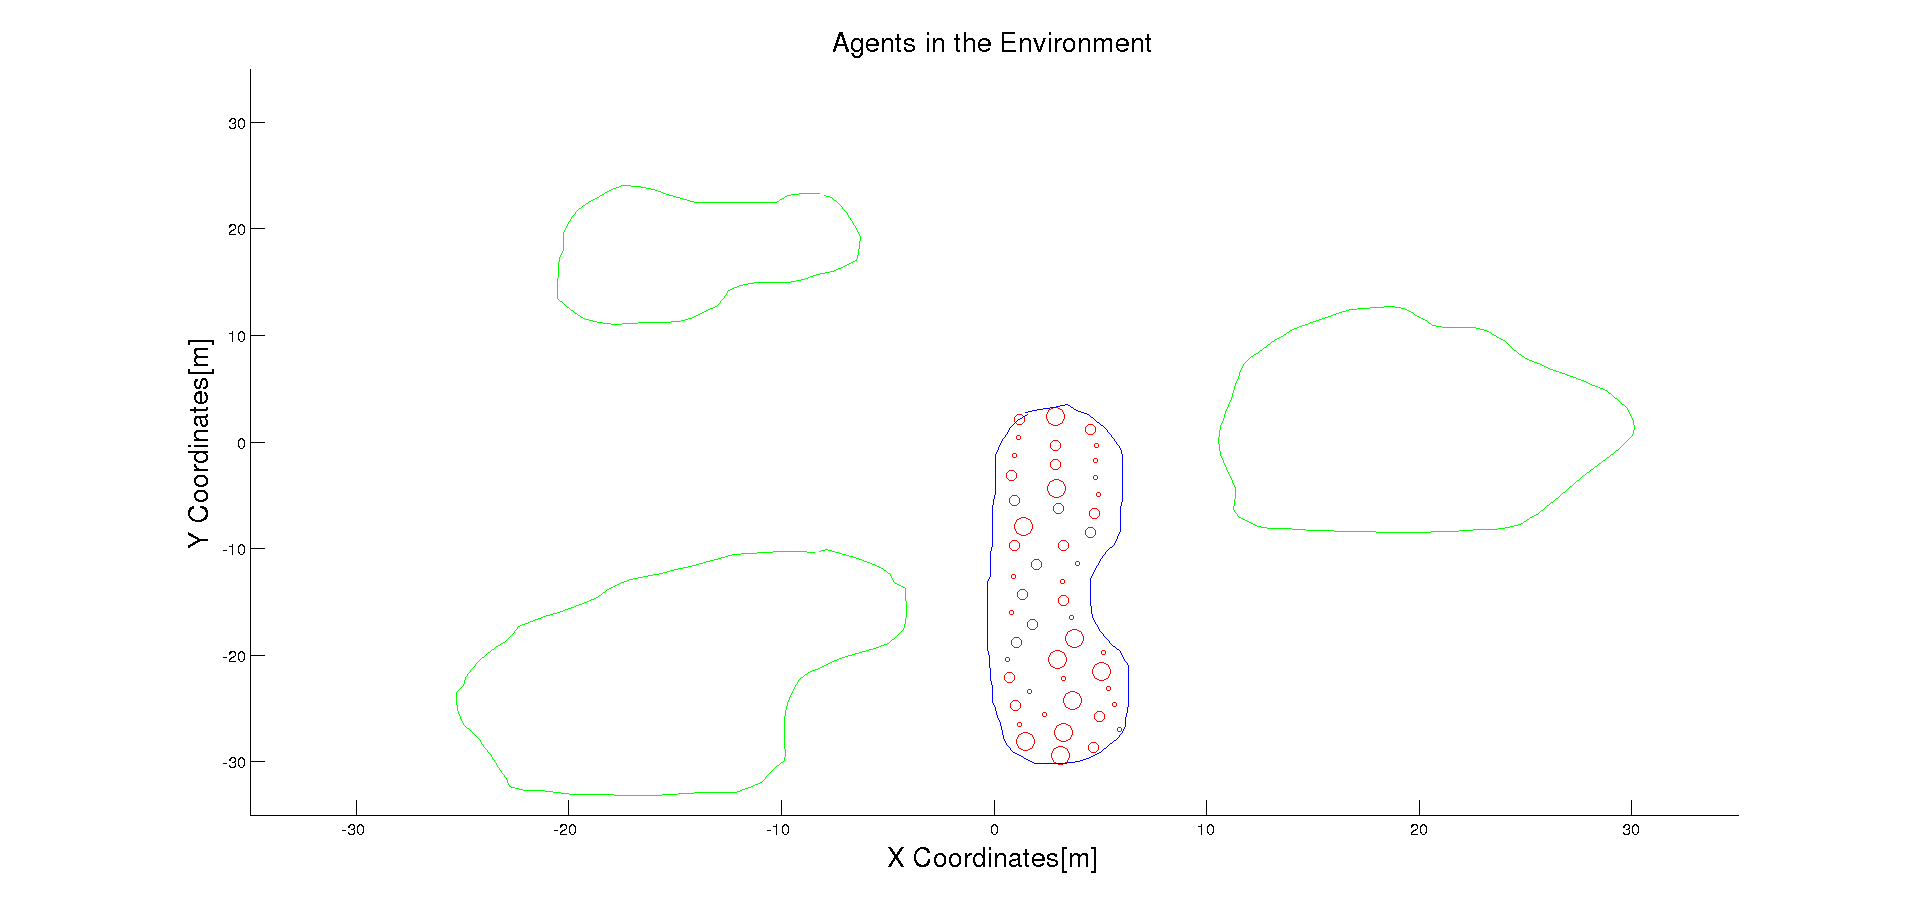
\includegraphics[scale = 0.40]{4}}
			\end{figure} 
			
			\begin{center}
				\captionof{table}{Performance Metrics for Shape - 4} \label{tab:title} 
				\begin{tabular}{||c| c |c |c ||}
					
					\hline
					\textbf{Energy Consumption[m]}  & \textbf{Settling Time[sec]} & \textbf{Topological Mesh Irregularity} & \textbf{Geometrical Mesh Irregularity}\\ 
					\hline
					1578 & 142 &  2.15& 0.56\\
					\hline
				\end{tabular}
			\end{center}
		
		
A simulation with multiple formation shapes sequentially is illustrated in Figure-xx.


	\begin{figure}[H]
		\caption{Multiple Formations}
		\centerline{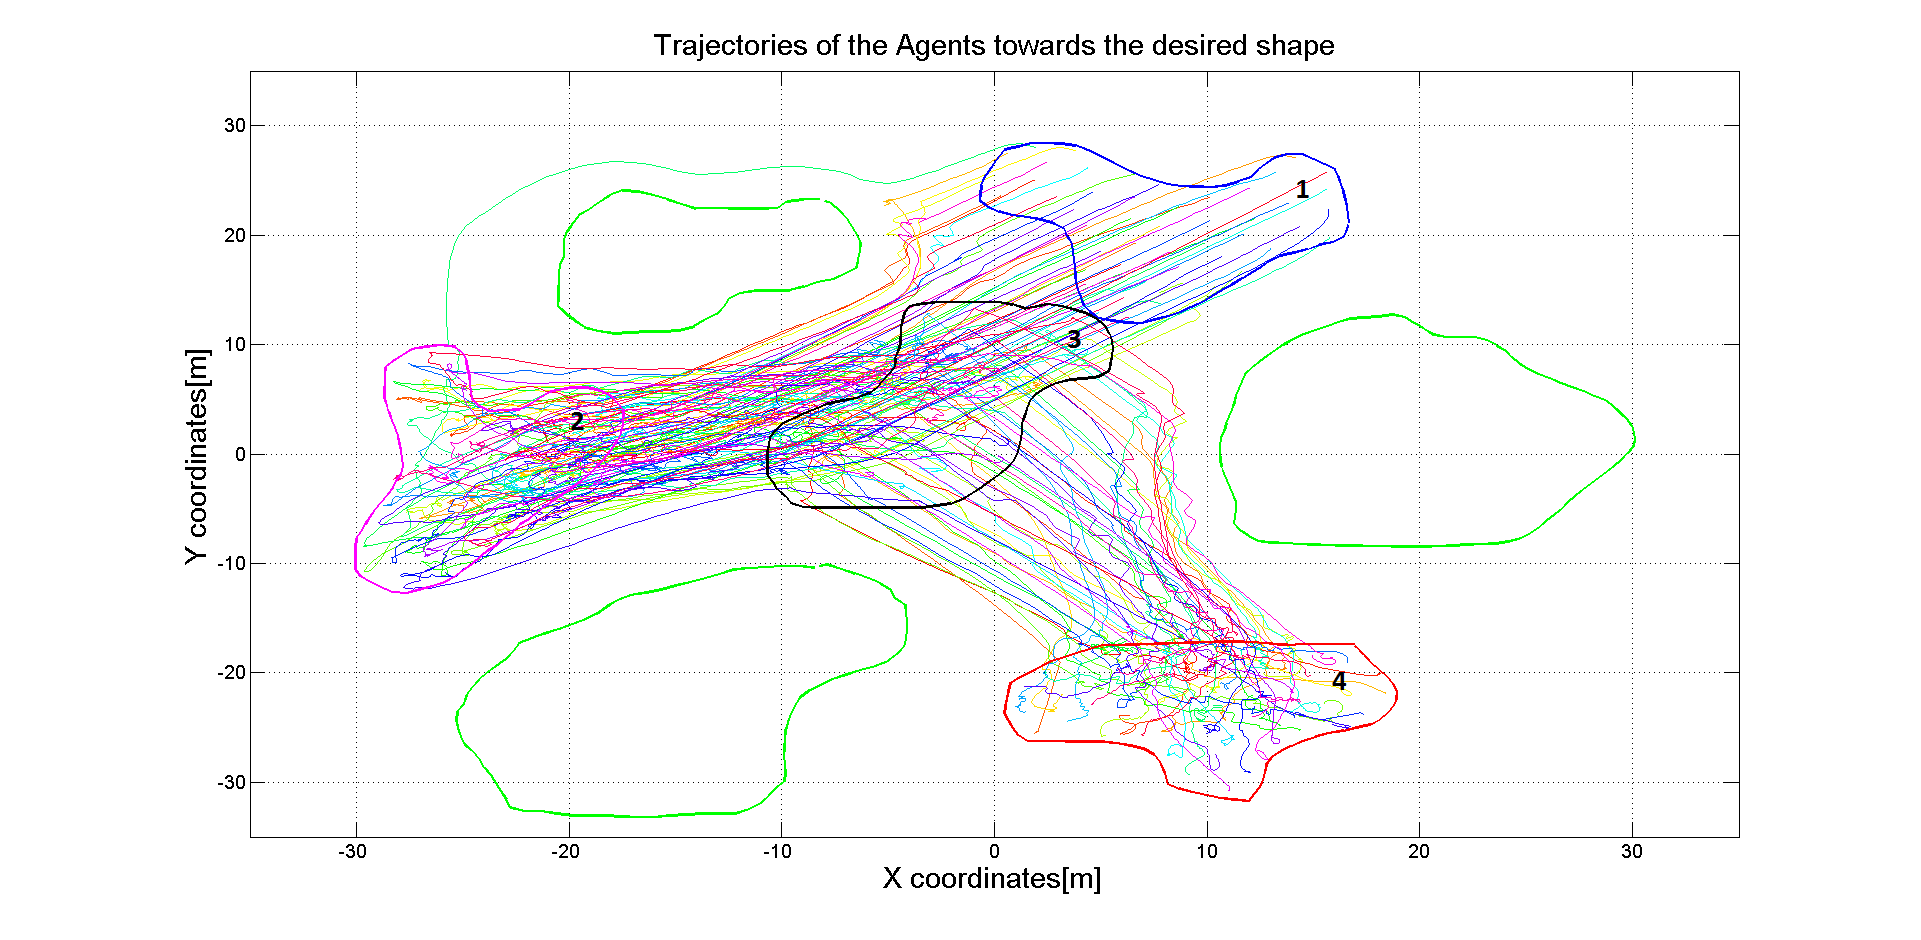
\includegraphics[scale = 0.45]{multiple_formation}}
	\end{figure} 
		
			\begin{center}
				\captionof{table}{Performance Metrics for Multiple Formation Shapes} \label{tab:title} 
				\begin{tabular}{||c| c |c |c ||}
					
					\hline
					\textbf{Total Energy }  & \textbf{Total Settling} & \textbf{Topological Mesh} & \textbf{Geometrical Mesh} \\ \textbf{Consumption[m]} & \textbf{Time[sec]}& \textbf{Irregularity Mean} & \textbf{Irregularity Mean} \\
					\hline
					4216 & 435 &  2.21& 0.68\\
					\hline
				\end{tabular}
			\end{center}
		